\chapterimage{Detector/DetFigures/VirgoTube.jpg} % Chapter heading image
%Einstein Telescope artist impression, copyright Nikhef
\chapter{Detector}
\label{chap:Detector}

%**********************************************
\section {Optical Layout}
% Authors A. Freise, S. Hild, R. Flaminio
\label{Sec:Layout}

\FloatBarrier
\label{sec:optlayout}

\tcb{from ET design  1.3.1}

\begin{wrapfigure}{r}{0.4\textwidth}
%\begin{figure}{H}
	\centering
		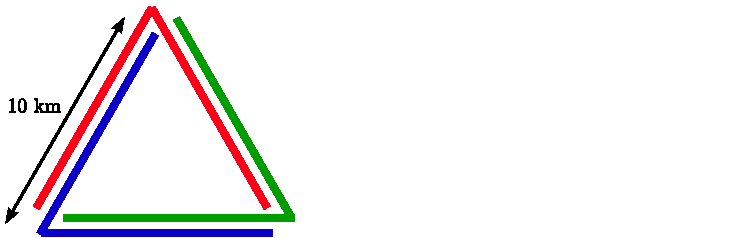
\includegraphics[width=0.3\textwidth]{Detector/Optics/Images//NestedDetectors.pdf}
	\caption{Three nested detectors in a triangular arrangement will 
	form the final Einstein Telescope geometry.}
	\label{fig:NestedDetectors}
\end{wrapfigure}
In its final construction stage the Einstein Telescope will consist of three nested detectors, which will be arranged in a triangular pattern as shown in figure\,~\ref{fig:NestedDetectors}. In contrast to the traditional L-shaped geometry of the first and second generations of gravitational wave detectors this arrangement is equally sensitive for both polarisations of the gravitational wave. Additionally it shows a more isotropic antenna pattern compared to the L-shaped detectors, as shown in figure\,~\ref{fig:response}. The overall frequency range covered will reach from a few Hertz to about 10\,kHz.

Each individual detector in turn will comprise two interferometers, one specialised for detecting low-frequency gravitational waves and the other one for the high-frequency part. The sensitivity goal for each interferometer is shown in figure\,\ref{fig:ET_sensitivity}. %\\ 
Each individual interferometer has a classical dual-recycled Michelson topology with arm cavities. This is a mature technique, well tested in laboratory experiments, and currently being set up for the second-generation detectors, Advanced LIGO and Advanced Virgo. More elaborate topologies like Sagnac interferometers or optical bars using Quantum Non-Demolition (QND) techniques do not promise significant advantages and have not yet reached the level of  maturity required for a project of this scale.\\



\tcb{from ET design  5.4}
This section describes the details of the ET optical layout, such as the laser beam sizes, beam shapes and distances between optical components inside the arm cavities and central interferometer including the power and signal recycling cavities. A schematic sketch of the optical layout of all core optical of the interferometers is shown in figure~\ref{Fig:Simple_ETv1}.
Constraints imposed onto the optical layout are briefly discussed in section~\ref{sec:opt_layout_class}, while  section~\ref{sec:xylophone} lays out the motivation for choosing a dual-tone xylophone detector. The optical layout of the arm cavities is discussed in detail in section~\ref{sec:arm_cavity_design}. Finally section~\ref{sec:opt_layout_CITF} describes the layout of the recycling cavities. 

\begin{figure}[p]
\centering
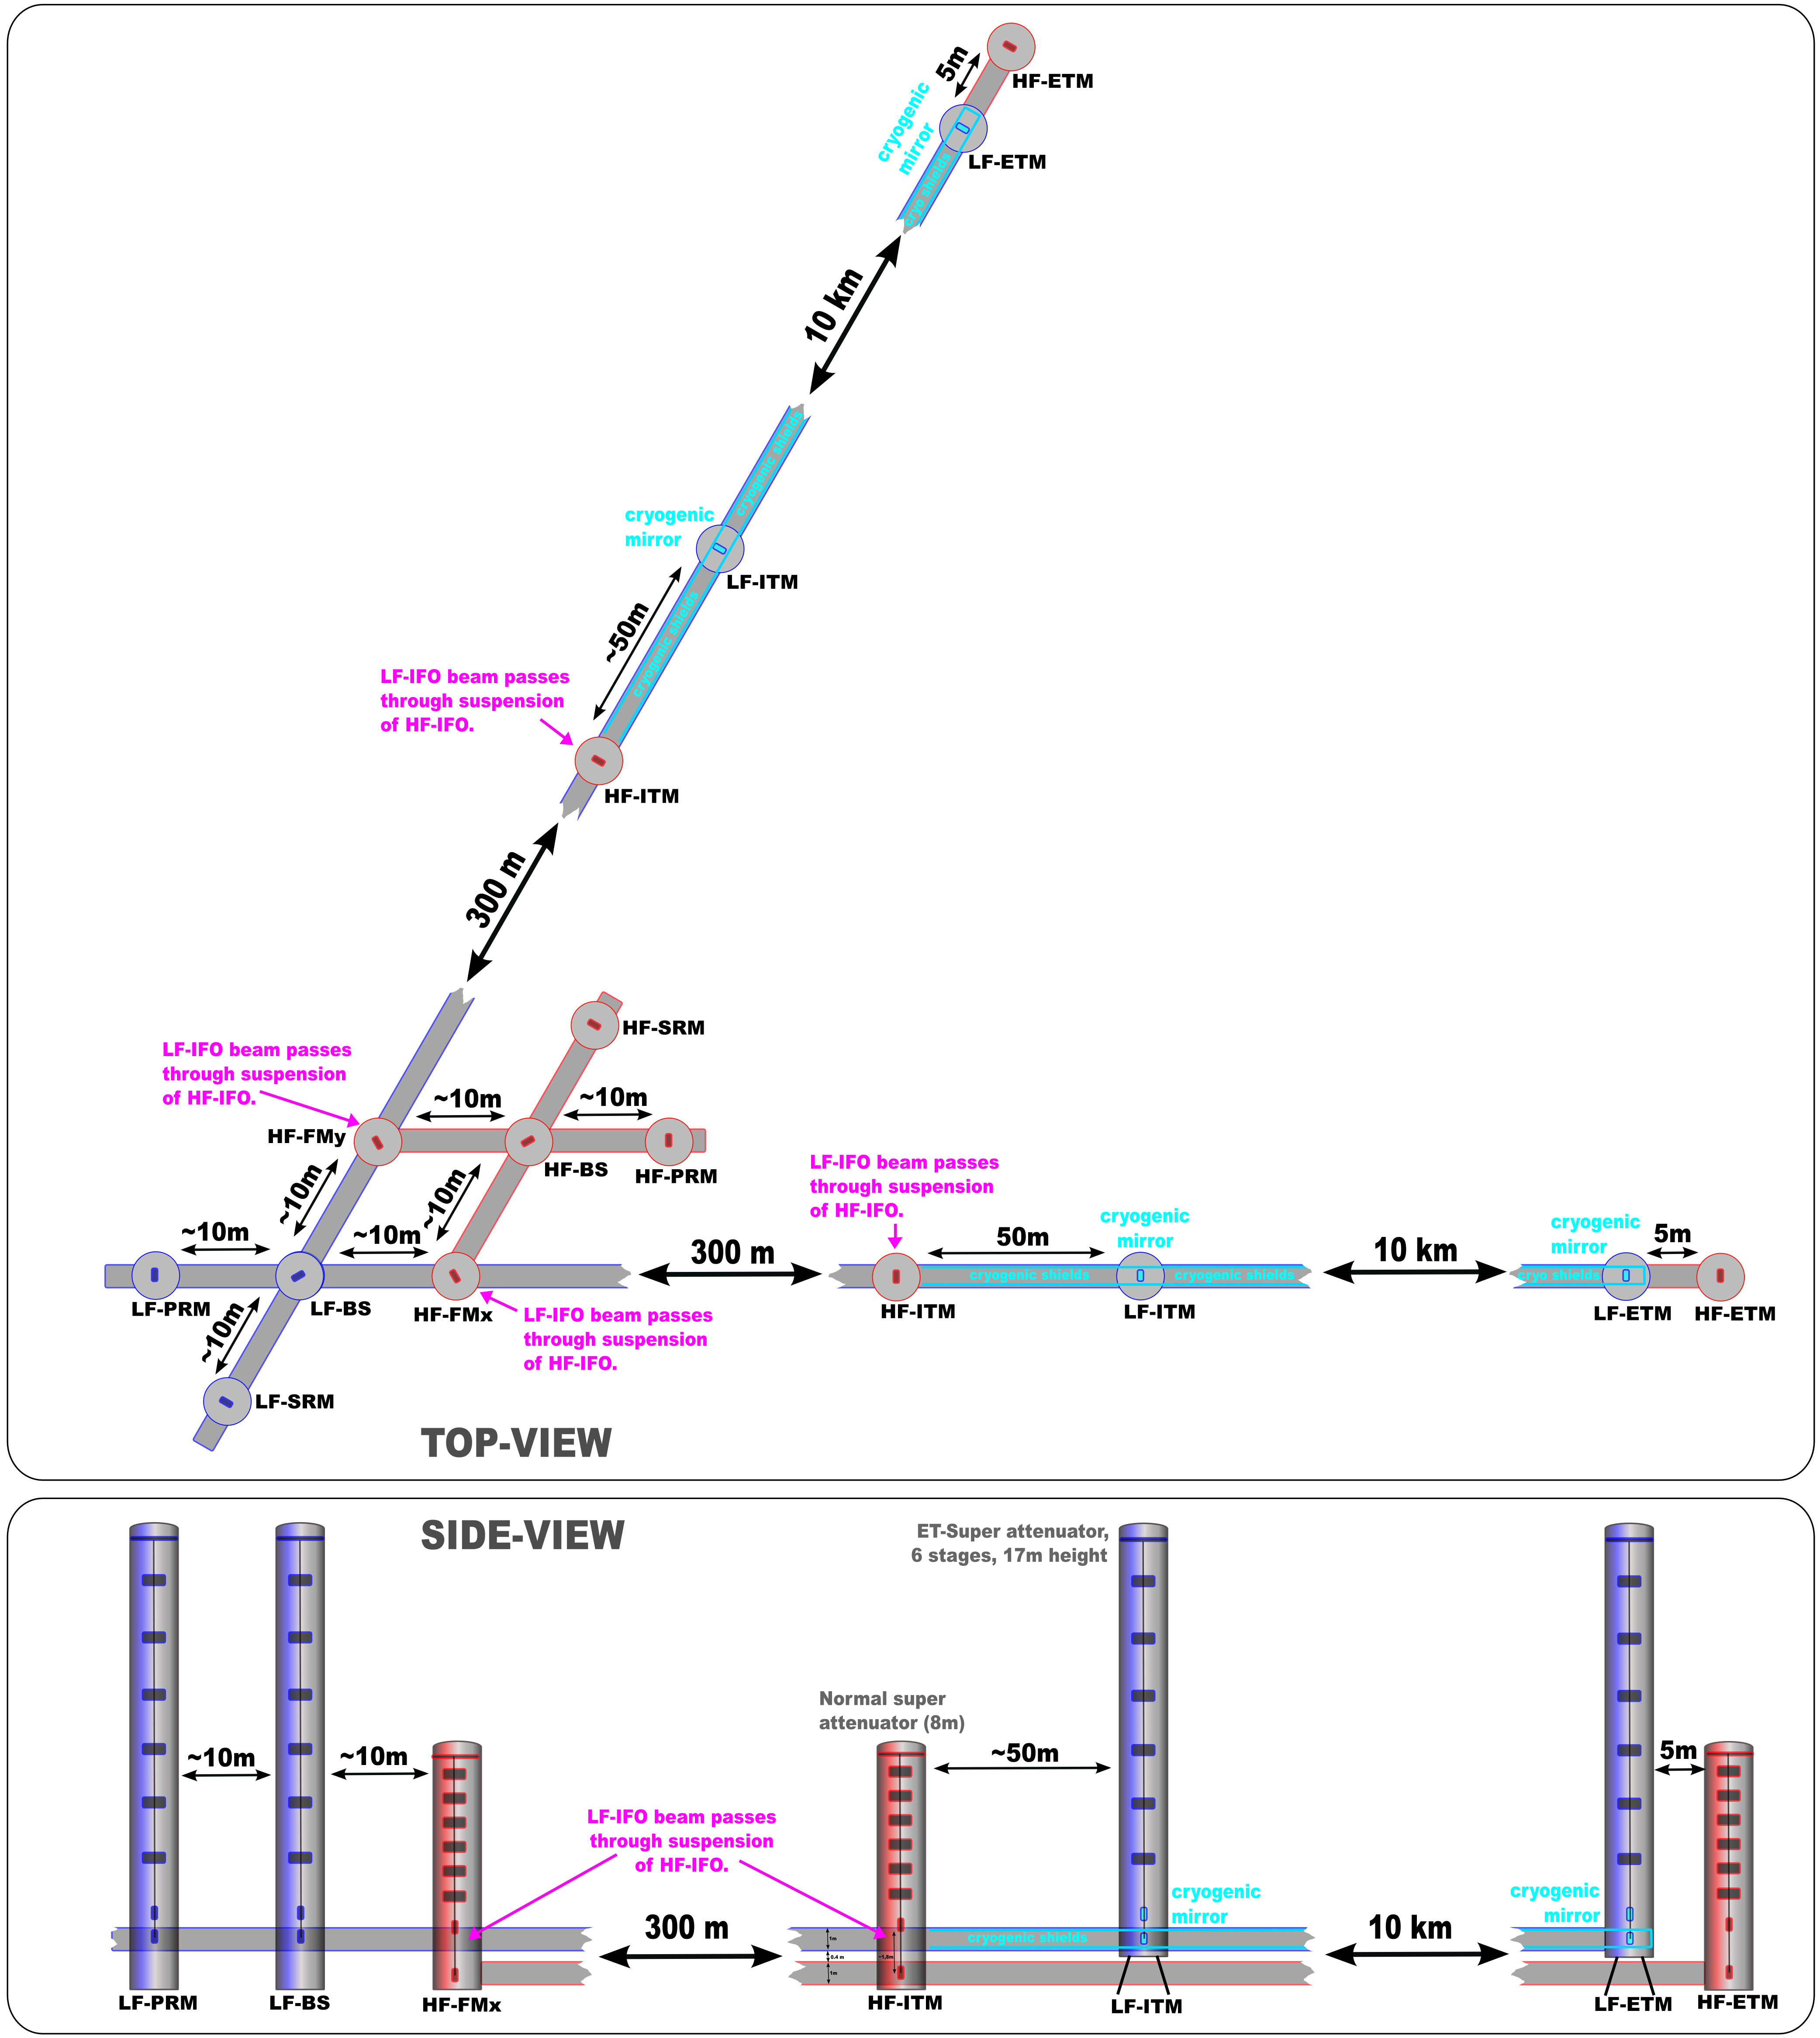
\includegraphics[width=1\textwidth]{Detector/Optics/Images/ET_April2011_v2.png}
\caption{Simplified drawing of the low and high frequency core interferometers of a single ET-detector. Injection and detection optics as well as filter cavities have been omitted for clarity. Please not that the complete ET observatory consists of three such detectors.%
}
\label{Fig:Simple_ETv1}
\end{figure}

\subsubsection{A xylophone design for ET}\label{sec:xylophone} 
\tcb{from ET design  5.4.2}
Spanning the detection band over four orders of magnitude in frequency, as is asked for third generation GW observatories such as ET, is technically extremely challenging: different noise types dominate the various frequency bands and often show opposite responses for different tuning of the same design parameter.

In the following we give some examples of fundamental issues of a broadband third generation interferometer that could be resolved by using a set of xylophone detectors:
\begin{itemize}
\item \textbf{High Power vs Cryogenic Temperature}: Using a single broadband ET observatory as described in \cite{HildETconventional} features the challenge of the simultaneous use of high optical power (a few megawatts) to achieve the required high frequency sensitivity and test masses at cryogenic temperatures in order to provide the required suppression of thermal noise. Even though tiny, the residual absorption of the dielectric mirror coatings deposits heat in the mirrors which is difficult to extract, without spoiling the performance of the seismic isolation systems. A possible solution for this problem would be to build a xylophone observatory consisting of a high frequency detector featuring high power and high temperature and a low frequency detector featuring low power and cryogenic temperatures.
\item \textbf{Shot Noise vs Radiation Pressure Noise}: Due to the fact that the shot noise contribution scales inverse with optical power, but the photon radiation pressure noise contribution on the other hand  scales proportional to the optical power, it will be hard to obtain the desired bandwidth with a single detector. Therefore, again it might be useful to split ET into a low-power low-frequency and a high-power high-frequency
companion.
\item \textbf{Mixing Interferometer Topologies}: Xylophone configurations would also allow us to mix alternative interferometer topologies, such as Sagnac interferometer \cite{Chen2003} and optical levers \cite{Khalili2002}, with the standard Michelson interferometer. For example one could imagine that ET upgrades would feature a standard high-frequency Michelson interferometer with a low-frequency optical lever as companion.
\end{itemize}

The xylophone concept was first suggested for Advanced LIGO,  proposing to complement the standard broadband interferometers with an interferometer optimized for lower frequency, thus enhancing the detection of high-mass binary systems
\cite{Shoemaker2001LIGOXylophone, Conforto2004}.

One may think that a xylophone might significantly increase the required hardware and its cost by the need to build more than one broadband instrument. However, such an argument does not take the technical simplifications that it would allow, the better reliability of simpler instruments, and the more extensive scientific reach allowable into account.

For example splitting a third generation observatory into a low-power, low-frequency  and a high-power high-frequency interferometer, has not only the potential to resolve the above mentioned conflict of photon shot noise  and photon radiation pressure noise, but also allows to avoid the combination of high optical power and cryogenic test masses. To reduce thermal noise to an acceptable level in the low frequency band, it is expected that cryogenic suspensions and test masses are required. Even though tiny, the residual absorption of the dielectric mirror coatings deposits a significant amount of heat in the mirrors. Since this heat is difficult to extract, without spoiling the performance of the seismic isolation systems, it imposes a limit on the maximum circulating power of a cryogenic interferometer.

\begin{figure}[thbp]
\centering
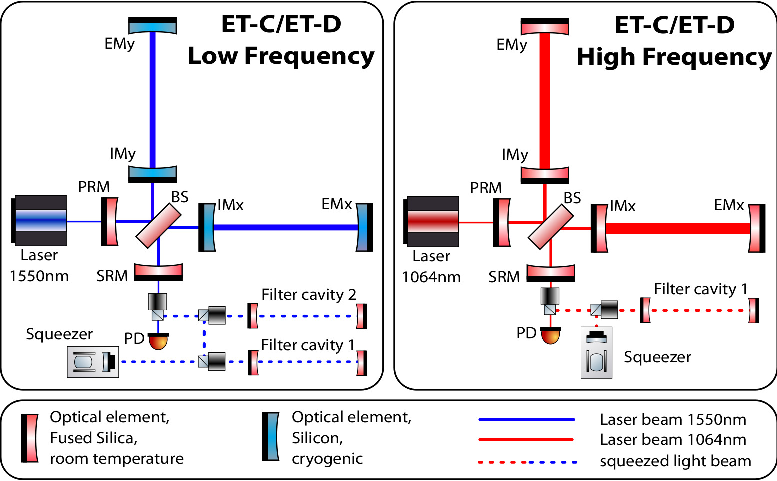
\includegraphics[width=0.8\textwidth]{Detector/Optics/Images/Layout_overview.pdf}
\caption{Simplified sketch of the ET low and high frequency core interferometers of a single ET-detector.}
\label{Fig:opt_lay_over}
\end{figure}

\begin{table}
\begin{center}
\begin{tabular}{l l l}
\hline
\hline
Parameter & ET-D-HF   & ET-D-LF \\
\hline
Arm length & 10\,km & 10\,km \\
Input power (after IMC) & 500\,W & 3\,W \\
Arm power & 3\,MW & 18\,kW\\
Temperature & 290\,K &  10\,K  \\
Mirror material & fused silica & silicon \\
Mirror diameter / thickness & 62\,cm / 30\,cm & min 45\,cm/ T \\
Mirror masses & 200\,kg & 211\,kg \\
Laser wavelength & 1064\,nm & 1550\,nm \\
SR-phase & tuned (0.0) & detuned (0.6)\\
SR transmittance & 10\,\% & 20\,\% \\
Quantum noise suppression &  freq.\ dep.\ squeez.& freq.\ dep.\ squeez.\\
Filter cavities & $1 \times 10\,$km  & $2 \times 10\,$km\\
Squeezing level  & 10\,dB (effective) & 10\,dB (effective) \\
Beam shape &  LG$_{33}$& TEM$_{00}$\\
Beam radius & 7.25\,cm & 9\,cm \\
Scatter loss per surface & 37.5\,ppm & 37.5\,ppm \\
Seismic isolation & SA, 8\,m tall & mod SA, 17\,m tall \\
Seismic (for $f>1$\,Hz) & $5\cdot 10^{-10}\,{\rm m}/f^2$ & $5\cdot 10^{-10}\,{\rm m}/f^2$  \\
Gravity gradient subtraction & none & none \\
\hline
\hline
\end{tabular}
\caption{Summary of the most important parameters of the ET-D high and low frequency interferometers. SA~=~super attenuator,  freq.\ dep.\ squeez.~=~squeezing with frequency dependent angle.\label{tab:summary14}}
\end{center}
\end{table}

The baseline for ET is a 2-band xylophone detector configuration, composed of a low-frequency (ET-LF) and a high-frequency (ET-HF) detector. Both interferometers are Michelson interferometers featuring 10\,km armlength and an opening
angle of 60 degrees.  Due to their similar geometry both detectors will share a single facility. Table~\ref{tab:summary14} gives a brief overview of the main parameters of the analysed low-frequency (ET-LF) and high-frequency (ET-HF) detector. Figure~\ref{Fig:opt_lay_over}   shows sketches of the corresponding core interferometers and the filter cavities. The full layout of the two core interferometers of a single ET detector is depicted in Figure~\ref{Fig:Simple_ETv1}.


% -------------------------------------------------------------------------------------------
\subsubsection{Arm cavity design}
\label{sec:arm_cavity_design}
\tcb{from ET design  5.4.3}

The size and shape of the laser beam inside the interferometer is defined by the surface shape of the cavity mirrors; the beam sizes at the arm cavity input mirrors (IM) and arm cavity end mirrors (EM) as well as the position of the cavity waist are determined by only two parameters, the radii of curvature (ROC) of IM and EM. Since inside the two Fabry-Perot cavities of the Michelson interferometer the GW interacts with the laser light, creating signal sidebands, the two arm cavities can be seen as the heart of the ET interferometers. The characteristics of the arm cavities have not only a high impact on the detector sensitivity and bandwidth, but also on the overall detector performance.

The choice of the beam size on the arm cavity mirrors is a trade-off process taking the following considerations into account:
\begin{itemize}
  \item For a given cavity length there is a minimal achievable beam size, which is determined by the divergence of the beam.
\item Above this minimal beam size, any further increase in beam size leads to and additional reduction of the various thermal noise contributions.
\item Finally the upper limit for the manageable beam size is given firstly by the maximum available mirror substrate size and secondly by the approaching of the cavity instability.
\end{itemize}

\textbf{Arm cavity mirror size}

A common method to define the mirror size is to demand the optical power loss due to clipping (light being lost because it `falls over the edge of the mirror') to be less than $1\,$ppm. The computation of the scaling factors is described in~\cite{Chelkowski2009} and results in:
\begin{center}
\begin{tabular}{|l|c|c|}
	\hline
	mode  & TEM$_{00}$ & LG$_{33}$\\
	\hline
	mirror radius to beam  radius & 2.63 & 4.31\\
	\hline
\end{tabular}
\end{center}

\textbf{Minimal mirror sizes for ET}

Using the currently discussed options for ET we can compute minimal mirror sizes for various options, by using $L=R_{C}$ resulting in $w_{\rm min}=\sqrt{\frac{L\lambda}{\pi}}$.
\begin{center}
\begin{tabular}{|l|c|c|}
	\hline
setup & min beam radius  & min mirror diameter \\
         & [cm] & [cm] \\
	\hline
LG$_{33}$, 1064\,nm  &  5.8      &  50.2     \\
	\hline
TEM$_{00}$, 1550\,nm  &  7.0      &   37.0    \\
	\hline
\end{tabular}
\end{center}

\textbf{Realistic mirror sizes for ET}

Using the minimal beam sizes is obviously not optimal in terms of thermal noise. Therefore we intend to push the beam sizes for ET towards the maximum feasible size, which corresponds to about 60\,cm substrate diameter for fused silica mirrors and 50\,cm for the silicon mirrors. Assuming 10\,km long arm cavities, we can derive the following arm cavity characteristics.

\begin{center}
\begin{tabular}{|c|c|c|c|c|c|c|c|c|}
  \hline
IFO & $\lambda$& beam shape & mirror diameter & $R_{\rm C}$ & $w_0$ &$z_0$ & $w$ & $z_{\rm R}$ \\
\hline
ET-HF & 1064\,nm & LG$_{33}$ & 62\,cm & 5691\,m & 2.51\,cm & 5000\,m & 7.2\,cm & 1859\,m\\
\hline
ET-LF & 1550\,nm & TEM$_{00}$ & 45\,cm &5577\,m & 2.9\,cm & 5000\,m & 9.0\,cm & 1698\,m\\
\hline
\end{tabular}
\end{center}

% ----------------------------------------------------------------------------------------------------

\FloatBarrier
\subsubsection{Central interferometer design}
\label{sec:opt_layout_CITF}
\tcb{from ET 5.4.4 design}

The central interferometer consists of the two recycling cavities and the central Michelson interferometer formed by the beam splitter and the arm cavity input mirrors. The design of the central interferometer is mainly determined by two constraints. First of all it should allow for the implementation of non-degenerate recycling cavities. Second, the central interferometer has to serve as mode-matching telescope for the arm cavities.

The non-degenerate recycling cavity design used by the advanced detectors (see Figure~\ref{Fig:Sec_Optics_AdvLIGO_IFO_Schematic}) can probably not be directly adapted for ET, because no beam splitter substrates of the required dimensions would be available. For example the high frequency interferometer featuring an opening angle of  60 degree would require a beam splitter with a diameter of 115\,cm.

Therefore we plan to investigate design options making use of input mirror substrates including a focussing lens with a focal length of 0.2 to 1\,km and shifting the input mirrors away from the beam splitter.  Figure~\ref{Fig:Simple_ETv1} illustrates how such a configuration would look like. Please note that the arm cavity mirrors are the only full sized optical elements and that beam splitter and recycling mirrors can be significantly smaller. In addition in this scenario no additional folding mirrors are necessary in the recycling cavities.

\textbf{Layout option for TEM$_{00}$, 1550\,nm}
\nopagebreak

The optical parameters of a possible solution based on a arm cavity length of $L=10$\,km and a TEM$_{00}$ mode at 1550\,nm are provided below:
\begin{itemize}
\item focussing element in or near the ITM with a focal length of $f=303$\,m
\item distance ITM--BS: 300\,m
\item distance BS--MPR: 10\,m
\item beam size on BS: 6\,mm
\item beam size on MPR: 3.4\,mm
%\item Rayleigh range in central interferometer: 6.3\,m
\end{itemize}

The recycling cavity formed by MPR and ITM has a length of 310\,m and a free spectral range of 484\,kHz. The round-trip Gouy phase is given by $\approx 9.6$\,deg which corresponds to a mode separation frequency of $25.8$\,kHz.

\textbf{Layout option for LG$_{33}$, 1064\,nm}
\nopagebreak

Using the same distances and focussing elements for the interferometer with a LG$_{33}$, 1064\,nm beam, we also obtain reasonable numbers:
\begin{itemize}
\item beam size on BS: 4.7\,mm
\item beam size on MPR: 2.7\,mm
%\item Rayleigh range in central interferometer: 6.7\,m
\item Gouy phase: 10.5\,deg
\item mode separation frequency:  28.1\,kHz
\end{itemize}

These layout options are not yet optimised but they show that a separation between beam splitter and input optics in the order of 300\,m represents a useful baseline. The numbers for the beam sizes at the beam splitter and recycling mirrors in both cases need to be checked against a detailed thermal noise computation.

Furthermore, the design needs to be evaluated for losses originating from astigmatisms inside the recycling cavities as well as for scattered noise issues.






\section{Optics and Interferometry}
% Authors R.Flaminio, A. Freise, S.Hild
\label{Sec:Optics}

\subsection{Core Optics and Coatings}
% Jerome
\label{Sec:CoreOptics}
This section focuses on the mirrors forming the arm cavities of the interferometer (IM and EM). Those optics, also called test masses, are the largest \tcb{(comment sthild:) by dimension} and most critical ones whose displacement noise can directly degrade the  \tcb{(comment sthild:) measurement of the } gravitational waves signals.

To ensure the best optics, the three ingredients of a mirror: substrate, polishing and coating will have to use state of the art technologies. An overview of current achievements and the core optics strategy for ET is presented in the following sections. The working temperature of the optics \tcb{(comment sthild:) better say "The temperature at which the mirror is operated  has ..." } have a strong impact on the technological choices to be made. 

\subsubsection{The substrate materials}

The substrate of the large \tcb{(comment sthild:) replace 'large' by 'ET main' } optics must meet some drastic \tcb{(comment mlorenzini: replace specifications with requirements)} specifications in term\tcb{s} of optical and mechanical specifications, moreover it should be available in large sizes with surfaces polished to the atomic level. Due to such constraints, \tcb{(comment sthild:) only a }few specific materials can be considered: fused silica for room temperature interferometer and silicon for cryogenic temperatures.\\

\paragraph{Fused silica} is the substrate of choice for all the current room temperature interferometers.  Due to its \tcb{(comment mlorenzini: Remove 'extensive') } extensive
use for first and second generation gravitational wave detectors, this material has been extensively characterised at room temperature. Moreover the polishing and coating are now well mastered for this material \cite{pinard2017mirrors}.

The operating wavelength of room temperature ET will be 1064~nm, the same as current advanced interferometers and well within the transparency region of fused silica. At this wavelength fused silica exhibits very low bulk optical absorption (below 1 ppm/cm) with high homogeneity of refractive index (relative optical path length < 0.1~nm/cm over the central part) and very low birefringence (around 1~nm/cm \cite{Degallaix:Large_optics_19}). The material can be isotropic in 3 dimensions which is ideal for the central beansplitter where laser beams are crossing the substrate at different angles.

In addition to its outstanding optical properties, fused silica presents a very low Brownian thermal noise at room temperature. Additionally, there exist techniques to fabricate quasi-monolithic suspensions based on pulled fused silica fibres and silicate bonding to further reduce the suspension thermal noise. These techniques have demonstrated their reliability and performances for years in the GEO600 detector \cite{plissi1998aspects} and so have been successfully implemented in the LIGO and Virgo detectors \cite{robertson2002quadruple,lorenzini2010monolithic}.

As a risk reduction for ET, the upgrade of Advanced Virgo, called Advanced Virgo+, will use test masses in fused silica of diameter 55~cm weighting 100~kg, that would be an essential step towards the optics for ET-HF which will be in the same material and with a diameter of 62~cm for 200~kg. 

In a nutshell, fused silica for large optical substrates presents the best optical and mechanical performances at room temperature and with very limited risks.\\


\paragraph{Silicon} is the favorite candidate material for the test masses for the cryogenic interferometer ET-LF. Compared to fused silica (and sapphire), silicon is not transparent at 1064~nm and so the operating wavelength of the detector has to be shifted to 1550~nm. 

Silicon has excellent mechanical and thermal properties and is easily available in relatively high quality due to the large market of the semiconductor industry. The coefficient of thermal expansion is zero at two special temperatures around 18~K and 125~K \cite{lyon1977siliconexpansion}. At these temperatures the contribution of thermo-elastic noise will therefore vanish. The mechanical loss of silicon has been studied by Q-factor measurements. It was experimentally shown that silicon bulk samples can reach mechanical losses as low as $1 \times 10^{-9}$ at 10~K. \cite{mcguigan1978siliconQ}.

The maximum available diameter and purity of silicon depends on the fabrication process. The two main growing processes for single crystal silicon used by the semiconductor industry are the Czochralski (CZ) and the Float Zone (FZ) methods. CZ silicon is grown from a silicon melt in a silica crucible. It results in relative large samples with a reasonable purity. The most dominant impurities in undoped CZ-grown silicon are carbon (typically 10$^{-18}$ cm$^{-3}$) and oxygen (typically up to 10$^{-19}$ cm$^{-3}$). 

In contrast, FZ silicon contains the same impurities but in much smaller concentrations (up to 10$^{-3}$ times smaller\tcb{(comment MGranata:) I would rather say "10$^{3}$ times smaller"}). During the FZ growth process, single or poly-crystalline silicon is remelted by means of inductive heating in vacuum or under an inert atmosphere. Impurities dissolve better in the melt than in the solid part. The re-crystallised material has therefore a higher purity than the initial one. By slowly sweeping the melt from one end to the other it is possible to purify in steps. The mechanism of inductive heating sets limits to the current production setups and leads to smaller available samples.

Using the CZ growth technique, silicon ingots up to 45~cm of diameter can be produced however 30~cm is still the dominant \tcb{(comment mlorenzini: perhaps replace "dominant" with "most common") } wafer diameter in the semiconductor industry. For FZ silicon the diameter is currently limited to 20~cm.

In the recent years, motivated by the possible use of silicon as test mass material, the optical properties of silicon have been thoughtfully characterised. Regarding the bulk optical absorption at 1550~nm, it was demonstrated the direct link between impurities concentration and the absorption \cite{degallaix2013abs_silicon}. For FZ silicon, absorption below 5~ppm/cm has been measured which is compatible with the ET-LF requirement. During the absorption studies, excess optical absorption at the surface of silicon was reported \cite{khalaidovski2013indication} which is likely linked to the polishing techniques used and not intrinsic to the material \cite{bell2017Sisurf}. According to the latest measurement \tcb{(comment mlorenzini: Perhaps a reference, if possible, should be added )}, magnetic Czochralski (mCz) growth technique would be the most suitable approach for ET as it can combine large diameter ingot (45~cm) with very low impurities since absorption around 20~ppm/cm has been achieved on one sample.

Thanks to the very low intensity of the laser beam in ET-LF, non linear effects such as two photon absorption \cite{bristow2007two} or Kerr effect are expected to be negligible in silicon.

Other caracterisations done in the framework of the Einstein Telescope include the measurement of thermo-optic coefficient at low temperature \cite{komma2012SithermoOptic} which is essential to derive the thermal lensing magnitude and the substrate thermo-refractive noise and also the birefringence \cite{kruger2015birefringenceSi} which is in the same order of magnitude as for sapphire. 

The choice of silicon substrate for ET-LF will be validated when it could be demonstrated that this material can come in large size (diameter of 450~mm\tcb{(comment MGranata:) everywhere else in this section, diameters are given in cm ----> 45 cm}) together with a very low optical absorption (order of several\tcb{(comment MGranata:) I would say "few" rather than "several"} ppm/cm) at 1550~nm. Silicon ingot made with mCz seems to meet those specifications on some samples but the repeatability has yet to be proven.

A backup substrate choice could be sapphire \tcb{(comment MGranata:) I would remove "as a candidate material for ET-LF", redundant here}as a candidate material for ET-LF. Sapphire is already used in the Japanese cryogenic interferometer KAGRA and hence extensive experience has been acquired on operating those mirrors \cite{Akutsu_2019} in cold conditions. As for silicon, very large sapphire boules \tcb{(comment mlorenzini: Consider replacing "boules" with "masses" or "bulks")} with excellent optical properties still have to be demonstrated.

\subsubsection{Surface polishing achievement}

The polishing capability will depend on the substrate material. Polishing of fused silica is well mastered thanks to current generation of room temperature interferometers and hence presents little risks. For the Einstein Telescope, the same flatness and roughness that was achieved \footnote{flatness inferior to 0.5~nm RMS and roughness below 0.1~nm RMS on the central part \cite{pinard2017mirrors}.} for Advanced detectors will be enough, albeit on a larger area. Due to the heavier substrate, special handling tools will have to be manufactured but according to the polishing companies, there is no showstopper. The large end mirrors of Advanced Virgo+ with a diameter of 550~mm and weighting 100~kg is \tcb{(comment mlorenzini: Replace "is" with "represent") } a pertinent pathfinder before the procurement of the ET mirrors.

Polishing of silicon does not carry any difficulties as this substrate material is heavily used for X-ray mirrors. Experiences from polishing companies indicate that silicon could be polished the same way as fused silica and similar performances on the flatness could be achieved (using also ion beam figuring to reach sub-nanometer flatness). The very low roughness is more challenging but 0.2 nm RMS could be achieved and is acceptable for ET. In a nutshell, the polishing of the large silicon substrates of ET is within the reach of the current technology.

Sapphire - the backup choice for low temperature test mass - is one of the hardest known material and has always been very difficult to polish. However, as demonstrated by the KAGRA detector, the outstanding surface quality of fused silica could also be reproduced on sapphire \cite{hirose2014sapphire} but at larger time and money-wise costs.

In summary, the polishing of the large substrates of the Einstein Telescope is within the current polishing capability and as such does not pose any challenge.

\subsubsection{Coating procurement}

Thin optical coatings, a few microns in thickness, must be added to the surfaces of the inteferometer mirrors to make them highly reflective. Since the thermal noise from these coatings will already limit the sensitivity of current room-temperature detectors at their most sensitive frequencies\tcb{(comment MGranata:) maybe recalling some references here would be useful, like the reference papers on Advanced Virgo and Advanced LIGO (Acernese et al CQG 2015, Abbott et al CQG 2015)}, it is essential to reduce coating thermal noise to achieve ET design sensitivity.

Highly-reflective coatings are usually composed of a stack of layers of alternating refractive index, with each layer having an optical thickness of a quarter of a wavelength. Using more layers or materials with a larger difference in refractive index \tcb{(comment MGranata:) I would rather say "with a larger refractive index contrast" (which is a ratio, not a difference)}results in higher reflectivity. Different layer thicknesses may be used to reduce thermo-optic noise\tcb{(comment MGranata:) a reference here?}, to optimise the coating thermal noise \tcb{(comment MGranata:) maybe add a reference here, A. E. Villar {\it et al.}, {\it Phys. Rev. D} {\bf 81}, 122001 (2010).}or to provide reflectivity at more than one wavelength.

The amplitude spectral density (ASD) of coating thermal noise can be approximated by\tcb{(comment MGranata:) maybe add a reference here, G. M. Harry {\it et al.}, {\it Class. Quantum Grav.} {\bf 19}, 897 (2002).}

\begin{equation}
x(f)=\sqrt{\frac{2 k_B T}{\pi^2 f}\frac{d}{w^2}\phi\left(\frac{Y_{\rm coat}}{Y^2_{\rm sub}} +\frac{1}{Y_{\rm coat}} \right)}\,
\label{equ:CTN}
\end{equation}

\noindent where $k_{\rm B}$ is the Boltzmann constant, $T$ the mirror temperature, $f$ the frequency, $d$ the coating thickness, $w$ the radius of the laser beam on the coating and $\phi$ the mechanical loss of the coating. $Y_{\rm sub}$ and $Y_{\rm coat}$ are the Young's moduli of the substrate and coating materials. This formula assumes that the bulk and shear mechanical loss angles of the coating are identical, that the mechanical loss is frequency independent and that the Poisson ratios of the coating and the substrate are zero. Further discussion of the validity of some of these assumptions is given below. While Eqn~\ref{equ:CTN} is often used to estimate thermal noise, it should be noted that the result can be as much as 30$\%$ different from the result given by the full formula which accounts for field penetration into the coating and does not neglect the Poisson ratios.

The main approaches to reducing coating thermal noise can be identified from Eqn~\ref{equ:CTN}:
\begin{itemize}
	\item Reducing the loss of the coating materials (lower $\phi$) e.g. by varying deposition parameters, post-deposition treatments or by developing alternative coating materials
	\item Reducing the required thickness of the coating (lower $d$) - using materials with a large contrast in refractive index results in fewer pairs of layers being required to provide the same reflectivity.
	\item Reducing the mirror temperature (lower $T$). While this directly reduces the thermal energy in the system, care is needed as the mechanical loss of many materials is strongly temperature dependent.
    \item Increasing the interferometer laser beam radius on the mirrors (larger $w$). This averages thermal motion of the coating over a larger area, reducing the noise. However, the laser spot size is limited by the radius of the mirror to keep scattering / diffraction losses at the edge of the mirror to an acceptable level.
\end{itemize}
\tcb{(comment MGranata:) I would suggest to add here the following sentence, right after the bullet list:
"Furthermore, the lowest coating thermal noise occurs when the coating Young’s modulus is matched to that of the substrate [x]."
[x] G. M. Harry {\it et al.}, {\it Class. Quantum Grav.} {\bf 19}, 897 (2002).}
Current detectors use coatings formed from alternating layers of silica (SiO$_2$) and titanta-doped tantala (TiO$_2$-Ta$_2$O$_5$)~\cite{Pinard2017,Flaminio2010,Harry2007}\tcb{(comment MGranata:) please add here the following reference:
M. Granata et al., https://doi.org/10.1088/1361-6382/ab77e9 . NB: Ref [131] is surely interesting for many reasons but is not about the actual coatings of aLIGO and AdV}. The loss of these coatings has been observed to increase at cryogenic temperatures, to a peak at $\sim$30\,K~\cite{Granata2013}. Similar loss peaks have been observed in single layers of SiO$_2$~\cite{Martin2014} and TiO$_2$-Ta$_2$O$_5$~\cite{Martin2009}, with the magnitude of the loss and the temperature at which loss peaks occur being strongly dependent on post-deposition annealing temperature~\cite{RobieThesis,Martin2010}. Current coatings are therefore not suitable for use at low temperatures \footnote{One study of an ion-beam sputtered silica/tantala coating did not show evidence of a loss peak at low temperature: however, the level of loss is still higher than required for ET-LF~\cite{Hirose2014}}.

\subsubsection{Coating thermal noise - full treatment}

Equation~\ref{equ:CTN} is an useful and convenient approximation of the magnitude of coating thermal noise. However, a material can have two independent loss angles, associated with shear deformations and `bulk' (volume change) deformations. These loss angles are assumed to be identical in Eqn~\ref{equ:CTN}: for many materials, this is unlikely to be a valid assumption. A more complete expression for coating thermal noise in terms of bulk and shear loss is given by Hong~\cite{Hong2013}. This treatment also shows that the thermal noise measured by an interferometer is more sensitive to the bulk loss angle than to the shear loss angle. For detailed thermal noise calculations, it is therefore important to know both the bulk and shear loss of the coating materials.

Equation~\ref{equ:CTN} ignores also the effect of the penetration of the laser beam into the coating stack. In reality, the sensitivity of the interferometer to thermal motion in a particular layer is dependent on that layer's position in the coating stack~\cite{Hong2013,gurkowski2010,gorodetsky2008,kondratiev2011}. While this usually results in a small correction of 10$\%$ or less, this effect must be taken into account when making accurate thermal noise predictions.

\subsubsection{coating requirements}

\paragraph{ET-LF}
To meet the goal of a factor of 25 improvement in sensitivity over aLIGO design sensitivity at 10\,Hz, ET-LF requires a reduction in coating displacement thermal noise by at least a factor of 10 with respect to the aLIGO design  sensitivity. Some of this improvement can be obtained from operating at low temperature and through the use of larger laser beam spots on the mirrors. The remainder of the improvement will need to come form the coating materials themselves. The most relevant material properties are the coating mechanical loss and the coating thickness (which is determined by the combination of refractive indices of the materials used in the coating stack). However, the elastic modulus of the coating (and of the mirror substrate) also contributes to the magnitude of the coating thermal noise.

For operation at 10\,K, after  accounting for the effect of  temperature and the effect of \tcb{(comment mlorenzini: Consider removing "the effect of")} larger beam size in ET-LF, a reduction in coating thermal noise ASD \tcb{(comment MGranata:) has this acronym been already used/explained above?"}by a factor of 1.24 must be obtained from improvements to the \tcb{(comment mlorenzini: Consider replacing "improvements to the" with "improved")}coating materials. When taking account of the substrate modulus effects, and assuming all coating properties except mechanical loss remain the same as in aLIGO, this translates to a factor of 3.8 reduction in coating loss compared to the loss of SiO$_2$/TiO$_2$:Ta$_2$O$_5$ at 10\,K.

\paragraph{ET-HF}
The target for ET-HF is a factor of 3.2 reduction in coating thermal noise ASD at 100\,Hz compared to aLIGO design sensitivity. Accounting for the slightly larger laser beam in ET-HF, this sets a requirement of a reduction in ASD by a factor of 2.7 from the coating materials. If we assume all coating properties except the mechanical loss remain identical, then a reduction in mechanical loss by a factor of 7.1 with respect to the aLIGO coatings would be required.

\paragraph{Other requirements}
In addition to meeting these thermal noise requirements, the coatings must have low optical absorption and low scattering. Low absorption is essential to minimise the heat-load on the cryogenic mirror. A target of 5\,ppm absorption was set in the original design study. Significantly lower absorption -- perhaps similar to the sub-ppm absorption of the current aLIGO and Advanced Virgo coatings -- may be required to enable the design of suspension fibres which can successfully extract the laser power absorbed by the mirror while also having acceptably low thermal noise~\cite{Cumming_2013}. Further studies in this area are likely to be required as detailed suspension designs are developed. 
For ET-HF, the coating optical absorption is also critical to limit the thermal expansion of the surface of the mirrors. The same absorption limit of 0.5~ppm similar to current detector will still hold.

Low scattering is required to minimise the optical round trip loss from the arm cavities and to prevent scattered light picking up additional phase noise (e.g. by reflection from the non-isolated beam tube) and coupling back into the interferometer beam. The target for scattering as optical loss is in the order of 10-20~ppm of loss per mirror.


\subsubsection{Coating design solutions}

\paragraph{multimaterial coatings} -- The use of so-called multimaterial coating designs has been proposed to enable the use of coating materials with higher optical absorption than can be tolerated in a traditional 2-material design~\cite{Yam2015,multimaterial2015}. In a multimaterial coating, the top few coating layers are made from low-absorption materials e.g. silica/tantala. These layers reflect the majority of the incident laser power, reducing the light intensity in the coating to a level where higher-absorption materials (e.g. aSi, in combination with a low-index material) can be tolerated in the lower part of the stack. This allows the low mechanical loss of materials such as aSi to be exploited, without significantly increasing the total absorption of the coating stack.

\begin{figure}
	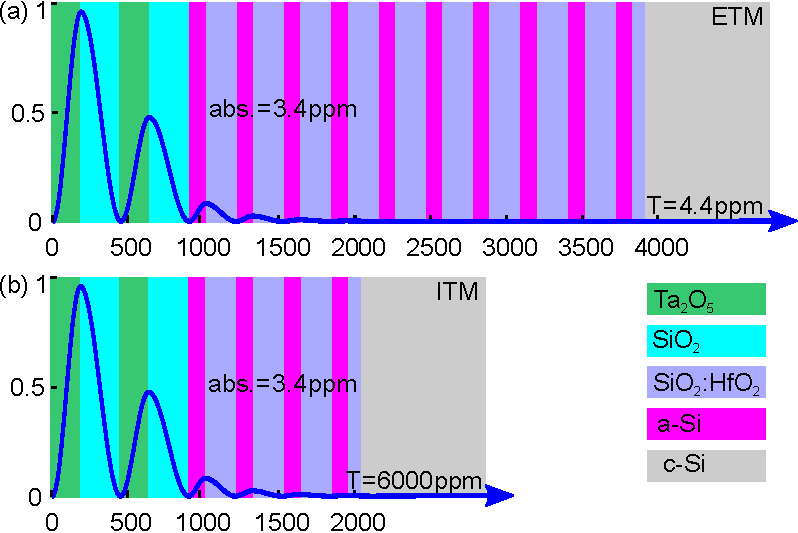
\includegraphics[width=12cm]{Detector/Optics/CoreOptics/Images/EFI_ETM_ITM_2.pdf}
	\caption{A multimaterial coatings design for (a) an ETM and (b) and ITM. This design uses an upper stack of SiO$_2$/Ta$_2$O$_5$ on top of a SiO$_2$:HfO$_2$/aSi lower stack~\cite{Craig_2019}. The blue lines show the electric field intensity as a function of depth in the coating.}
\label{fig:coatings:mulitmat}
\end{figure}

Several possible multi-material designs have been proposed to date~\cite{Steinlecher_2017,ion_plating,Pan_2018,Birney_2018,Craig_2019}\tcb{(comment MGranata:) there are 2 undefined references here}, including one that theoretically just meets the ET-LF coating thermal noise target for an optical absorption of 3.4\,ppm~\cite{Craig_2019}. This coating design relies on a level of absorption in aSi films which has been observed~\cite{Birney_2018}\tcb{(comment MGranata:) undefined reference here}, but has not yet been demonstrated reproducibly or on the scale required for ET.

Experimental verification of the performance of prototype multimaterial coatings has been reported~\cite{Gras_GWADW,Kinley_Hanlon_Warsaw} -- although it should be noted that a coating meeting the thermal noise and optical requirements of ET-LF has not been tested to date.

\paragraph{nanolayer coatings} -- Annealing at high temperatures is desirable to reduce the mechanical loss and optical absorption of many coatings: however, the onset of crystallisation (which results in higher mechanical loss and increased optical scattering) can limit the annealing temperature which can be used\tcb{(comment MGranata:) consider replacing "used" by "reached"}. The nanolayer approach involves making a single coating layer out of an array of thinner layers of two materials~\cite{Pan2014,Sankur1989}. This substructure can act to constrain crystallisation in the material, allowing higher annealing temperatures and lower mechanical loss to be achieved. This has been demonstrated for a high-index coating layer formed from a substructure of titania/silica nanolayers~\cite{Pan2014}.

More recently, it has been shown that the cryogenic loss peaks observed in silica coatings can be eliminated by using silica nanolayers separated with titania 'blocking' layers~\cite{Kuo2019}. Nanolayer coatings may therefore provide an excellent way to gain better performance from amorphous oxide materials at low temperatures. An important consideration for nanolayer coatings is to define the precision and uniformity with which each nanolayer needs to be deposited.\tcb{(comment MGranata:) I suggest adding here the following sentence: "To date, the deposition
of a full high-reflectivity coating embedding composite nanolayers has yet to be
achieved."}

\paragraph{Coating structure and mechanical loss} -- Significant progress has been made in predicting the cryogenic mechanical loss of coating materials computationally using molecular dynamics simulations~\cite{Hamadan2014,Trinastic2016,Billman2017}\tcb{(comment MGranata:) Please, add here also the following reference: F. Puosi et al., Phys. Rev. Res. 1, 033121 (2019).} and to obtain agreement with trends and magnitudes of experimental loss data.

Other structural work has shown the room-temperature loss may be correlated with medium-range order in Ta$_2$O$_5$ coatings, with more ordered structures and lower loss resulting from heat-treatment~\cite{Hart2016}. The evidence points towards the possibility that the same structural features responsible for low loss at room-temperature may be responsible for higher loss at cryogenic temperature. Raman spectroscopy studies have identified correlations between the ring structures and loss in silica coatings~\cite{granata2018correlated}. \tcb{(comment MGranata:) Please, add here also the following sentence and reference: "Very recent work has shown that a correlation exists between optical properties and internal friction in high-index oxide coatings [x]." 
[x] Amato et al., Sci Rep 10, 1670 (2020).}

Recently, evidence that specific structural units may correlate with lower loss has been found, in particular glassy structures with a high degree of corner-sharing, rather than edge or face sharing, between neighbouring tetrahedrons~\cite{Parsai2019}. This allows the structures of potential coating materials - many of which are well characterised - to be examined, and promising materials exhibiting a high degree of corner sharing to be identified and further investigated.

This increased understanding of the links between atomic structure and coating loss is a highly useful tool for developing lower-loss coatings.

\subsubsection{Possible coating materials}

\paragraph{Amorphous silicon} --  Amorphous silicon has low mechanical loss at cryogenic temperatures~\cite{Liu_1997,Murray2015}\tcb{(comment MGranata:) undefined reference here}, and has a relatively high refractive index, allowing thinner coatings -- with correspondingly lower thermal noise -- to be made. Mechanical loss as low as 2$\times10^{-5}$ has been observed in aSi coatings at room temperature and at cryogenic temperatures, and even lower loss is possible for coatings deposited at elevated temperature~\cite{Liu2014}. Elevated temperature deposition allows the aSi to form an `ideal glass' structure -- a low entropy amorphous state with very low loss.

While aSi is a very attractive material for thermal noise reasons, the optical absorption has historically been too high for use in gravitational wave detectors. Commercially grown ion-beam sputtered aSi coatings can have optical absorption of 1000 to 10000\,ppm at 1550\,nm (for a room-temperature HR stack made of aSi and SiO$_2$)~\cite{Steinlechner2016,Birney2018}. Significantly lower absorption can be achieved using a commercially available ion plating technique~\cite{ionplating}, and even lower again via electron cyclotron resonance (ECR) ion-beam sputtering~\cite{Birney2018}. The absorption of aSi tends to be significantly lower -- between a factor of 5 and 10 -- at $\sim$2000\,nm than at 1550\,nm~\cite{ionplating}. Operating ET-LF at a wavelength close to 2000\,nm may therefore be desirable to enable the use of aSi coatings for thermal noise reduction. While the absorption of the best aSi measured is still too high to allow a traditional aSi-based coating to be used, the incorporation of aSi layers into a mutimaterial coating design can allow significant thermal noise improvements while minimising the absorption contribution of the aSi layers.

aSi may also be a candidate material for a room-temperature coating. However, without further reductions in optical absorption, this is significantly more likely for a laser wavelength of 1550\,nm than for 1064\,nm, due to the higher optical absorption of aSi at 1064\,nm. However, it is interesting to note that some thermal noise reductions may be possible using aSi in a multi-material design at 1064 nm.

\paragraph{Silica coatings} \tcb{(comment MGranata:) I suggest changing the name of this paragraph to "Fluorides" and adding some text at the end of it, see below. Another option could be "Alternative cryogenic low-index layers"}-- For room-temperature detectors, efforts have largely focussed on improving or replacing the high-index coating layers which currently dominate the thermal noise. The current low-index material, silica, has a relatively low loss (as low as 4.5$\times10^{-5}$) at room temperature\tcb{(comment MGranata:) a most recent analysis shows that it is rather $\sim$2 $\times10^{-5}$: M Granata et al., https://doi.org/10.1088/1361-6382/ab77e9}. However, the loss of silica films increases significantly at cryogenic temperatures~\cite{Martin2014} - with both the structure and the magnitude of the loss being strongly dependent on post-deposition heat-treatment temperature~\cite{RobieThesis}. Therefore alternative low-index materials to silica will be required at for cryogenic coatings. A lower-loss low-index material is also likely to be required to achieve the required reduction in coating thermal noise at room temperature, although at the moment thermal noise remains dominated by the high index Ta$_2$O$_5$ layers. The room-temperature loss of silica can be further reduced by annealing at higher temperatures up to 900$^\circ$C\tcb{(comment MGranata:) please add here the reference supporting this statement: A. Amato et al., J.  Phys.: Conf. Series 957, 012006 (2018).}. In current coatings, crystallisation of the tantala layers prevents annealing above $\approx 600^\circ$C\tcb{(comment MGranata:) please add here the reference supporting this statement: A. Amato et al., J.  Phys.: Conf. Series 957, 012006 (2018).}.

\tcb{(comment MGranata:) I suggest adding the following text here: "In order to replace SiO$_2$ layers with lower-index materials, the optical properties and the internal friction of sputtered MgF$_2$ and AlF$_3$ coatings have been characterized at room temperature [Granata20]. Lower refractive index, higher optical abosrption and internal friction have been observed. Work is ongoing to characterize the impact of annealing on absorption and internal friction, at room and low temperature, for possible implementation in future cryogenic detectors like ET-LF."
[Granata20] M. Granata et al., Appl. Opt. 59, A229 (2020).}.

\paragraph{Silicon nitride} -- Silicon nitride films can have mechanical loss in the order of $1\times10^{-5}$ around 10\,K~\cite{Liu_2007} for a film on a substrate, and less than $1\times10^{-6}$ for substrate-free films~\cite{Southworth2009}. The refractive index of SiN is relatively low, making it of interest as a low-index material for use alongside aSi~\cite{Pan2017,ionplating}. Studies have shown that the exact composition of SiN films can strongly affect the refractive index, optical absorption and mechanical loss. Large enough refractive index variations can be obtained by changing the composition to potentially allow SiN to be used for both the high and low index coating layers. The optical absorption of SiN can be similar to the best aSi commercially available aSi films~\cite{Pan2017,Steinlechner2017}. A multimaterial design has been proposed to further reduce this absorption to below 5\,ppm for an HR stack ~\cite{Pan_2018}, although this design does not meet the ET-LF thermal noise requirements. 

Low mechanical loss has also been demonstrated in silicon nitride at room temperature and in sputtered films~\cite{Amato_2018}\tcb{(comment MGranata:) please replace this reference with a most recent one with updated data: M. Granata et al., Appl. Opt. 59, A229 (2020).}. Silicon nitride can withstand annealing at higher temperatures than tantala, \tcb{(comment MGranata:) please add here: "up to 900 $^{\circ}$C [x],"
[x] M. Granata et al., Appl. Opt. 59, A229 (2020).} allowing for the possibility of high-temperature annealing to produce a low loss Si$_3$N$_4$/SiO$_2$ coating.

\paragraph{Silica-doped hafnia} -- HfO$_2$ coatings have been shown to have lower cryogenic mechanical loss than SiO$_2$ and Ta$_2$O$_5$, but the material partially crystallises on annealing, resulting in poor optical properties~\cite{Abernathy_2011}. Doping HfO$_2$ with SiO$_2$ prevents crystallisation due to annealing, without increasing the cryogenic loss. With reasonably low optical absorption, SiO$_2$-doped HfO$_2$ shows promise for use as a low-index coating material to use with \tcb{(comment MGranata:) consider replacing "to use with" by "together with".}high-index aSi layers at cryogenic temperatures~\cite{Craig_2019}. This material is not of interest for ET-HF due to a relatively high room-temperature loss~\cite{CraigThesis}.

\paragraph{Alumina} Al$_2$O$_3$ coatings can have a lower mechanical loss than SiO$_2$ at cryogenic temperatures~\cite{RobieThesis}. While the refractive index is not as low as for SiO$_2$, this material may be of interest for use as a low-index material alongside materials like aSi which has a particularly high index. There has been interesting evidence that alumina coatings deposited at elevated temperatures can have significantly lower cryogenic loss than coatings which are heat-treated after deposition (REFERENCE - Abernathy?)\tcb{(comment MGranata:) I agree that a reference to the work of Abernathy et al. would be appropriate here, though -to my knowledge- only restricted-access LVC presentations are available to date?}.

\paragraph{Other amorphous coatings}
Improved amorphous oxides, with improvements being targeted using improved knowledge of the links between loss and structure, remain of interest for room-temperature coatings in particular. Options under investigation \tcb{(comment MGranata:) I can suggest a review article to be possibly cited here, covering all these options: M. Granata et al., Appl. Opt. 59, A229 (2020).}include studies of doping/mixing to increase crystallisation temperature and enable high-temperature annealing, the formation of ideal glass states using elevated temperature deposition and identifying materials with a high degree of corner-shared structural units. 

\paragraph{Crystalline coatings}

Multilayer single-crystalline coating materials can be grown epitaxially and can have very low mechanical loss. GaAs/AlGaAs crystalline coatings have been studied extensively, with a loss of 5.4$\times10^{-6}$ demonstrated at 20\,K for substrate-free resonator~\cite{Cole_2012}. Room temperature thermal noise measurements in small cavities are consistent with a coating loss of 4$\times10^{-5}$ at room temperature, and excellent optical absorption and scattering have been observed at wavelengths around 1550\,nm and 2000\,nm~\cite{Cole_2016}. AlGaAs coatings are grown on GaAs substrates, and would require to be transferred and bonded to a silica or silicon mirror - a process that is well-developed, at least for relatively small mirrors\tcb{(comment MGranata:) I do not agree with this sentence, since {Penn2019} has shown that there are relevant bonding issues even with 3" samples. I suggest replacing by "a process that might need further development"}. Currently the maximum available diameter of GaAs wafers is 20\,cm, which is not large enough for ET mirrors. However, there is now industrial interest in the production of larger GaAs wafers, with progress towards wafer diameters up to 30\,cm.\tcb{(comment MGranata:) I suggest that at some point in this paragraph above, the risk of many defects (up to 50 microns), showed again by {Penn2019}, should be also mentioned.}

Recent work suggested that the bulk loss of AlGaAs may be significantly higher than the shear loss~\cite{Penn2019}. Since the total coating thermal noise is more sensitive to bulk than to shear loss, this requires more investigation. It should be noted that low thermal noise has been directly measured in AlGaAs coatings, although so far only on relatively small mirrors with small laser beams~\cite{Cole_2013}.

GaP/AlGaP crystalline coatings have also been investigated~\cite{Lin}, with mechanical loss as low as 2.5$\times10^{-5}$ measured at 20\,K~\cite{Cumming_2015}. This material is of interest as it is lattice-matched to silicon and can be grown directly onto silicon substrates, potentially removing the need for substrate transfer (although growing a coating on an ET-sized mirror is unlikely to be feasible). Measurements of an initial highly-reflective stack showed high optical absorption of 2.3$\%$~\cite{Lin_2015}: however, there may well be scope to reduce this absorption e.g. be reducing impurities in the coating materials and coating chambers.\tcb{(comment MGranata:) I suggest to add also the following: "Also, to
date, the number of layer in a high-reflectivity coating is limited [x], resulting in a limited reflectivity."
[x] Cumming et al., Class. Quantum Grav. 32, 035002 (2015).}

For both GaAs/AlGaAs and GaP/AlGaAs coatings, the difference in refractive index between the two materials is relatively small, and so many layers are required to provide high reflectivity, reducing some of the thermal noise improvements due to the low loss.

\paragraph{Coating deposition}
The ET mirrors will be significantly larger than current gravitational detector mirrors, and ensuring the required coating uniformity over larger diameters will require development of coating deposition facilities. This development is already underway at the state-of-the-art coating facility at LMA. Problems with point absorbers and with bubbles - possibly of the sputtering ions used to deposit the coating - have been observed in the coatings for Advanced LIGO and Advanced Virgo: work to understand the origin of these defects and to eliminate them is a priority. \tcb{(comment MGranata:) I suggest to remove "and with bubbles" from the sentence above and to add the following sentence at the end of this paragraph: "Also, the occurrence of bubble-like defects limiting the annealing temperature of different coatings (high-index oxides) has been observed in multi-layer high-reflective stacks, work is currently ongoing also to understand and solve this issue".}

\paragraph{Strategy for ET}

Significant progress has been made towards development of coatings suitable for use at low temperatures in ET-LF. There are several highly-promising routes to meeting the coating thermal noise and optical absorption requirements. However, further study is required of the potential trade-off between coating absorption requirements, suspension thermal noise, ultimate mirror temperature and substrate thermoelastic noise -- and it seems likely that lower absorption than 5\,ppm may be required.

Achieving significant reductions in coating thermal noise at room temperature may be more challenging than at low temperature. Work in this area is ongoing, both for ET and for upgrades to the aLIGO and Advanced Virgo detectors, and there are several promising avenues\tcb{(comment MGranata:) consider replacing "avenues" by "options"}. One limitation is that some coatings which show promise for the low-temperature detector at 1550\,nm have significantly higher optical absorption at 1064\,nm, the wavelength envisaged for the room-temperature detector. Detailed studies of the benefits of operating the room-temperature detector at 1550\,nm may be of interest, as this may allow significant thermal noise reductions through the use of e.g. aSi-based coatings.

%A thin coating (few micrometers thick) is added to the polished substrates to create the optical function. For the arm cavities, the coating is a very high reflective reflector made of layers of alternate materials to form a Bragg grating. The constraints on the coating are extremely stringent as the coating must induce minimal displacement noise as well as very low optical loss.

%More specifically the coating Brownian thermal noise is the dominant source of noise and is expected to limit the sensitivity of Advanced detectors. So to further increase the detection range, intense worldwide research is currently lead to find better materials for the coating \cite{granata2019progress}. The Einstein Telescope will fully benefit from this research. 

%It is worth noting that compared to current interferometers, the impact of thermal noise on the ET noise budget is mitigated thanks to longer arm length and larger beam size.

%\paragraph{Room temperature interferometer}

%ET-HF share the same coating specifications as the Advanced LIGO + upgrade, to be operated around 2022 (a coating loss angle reduced by a factor 3 compared to current mirrors). So far no coating formulas or recipe have been found to match this requirement on large size, however people are optimistic that at the time of ET such coating would be present and well tested.


%\paragraph{Cryogenic interferometer}

%The cryogenic interferometer benefits from the lower temperature as the displacement induced by thermal noise scales as the square root of the temperature. A recent design using a multi-material approach (with the usual Ta$_2$O$_5$ and SiO$_2$ layers on top of a stack SiO$_2$:HfO$_2$ and amorphous silicon layers) has shown to meet the requirement for ET-LF \cite{craig2019mirror} for both the coating thermal noise and the optical absorption. 


\paragraph{Other core optics}

Central interferometer optics such as Power and Signal Recycling Mirrors (PRM and SRM) or beamsplitter will be smaller in size (diameter in the order of 10~cm) and at room temperature. Fused silica is hence the preferred material for the substrates. The coating will use the same materials as for ET-HF to benefit from state of the art deposition process. The procurement of those optics does not represent any challenges and will be straightforward.

\subsection{Light sources}
\label{Sec:Lasers}
% Author: Benno Willke?

\subsection{Quantum noise reduction}
\tcb{ET design, 5.5, also D3 (filter cavity)}
% interferometer configuration, squeezing, 
\label{Sec:Squeezers}
% Author: H Vahlbruch?, S. Danilishin?, Jean-Pierre Zendri?

%\subsection{Auxilliary Optics}
%\input{Detector/Optics/AuxOptics/AuxOptics.tex}

\subsection{Interferometer control}
% Hartmut Grote
\tcb{does not exist yet}



To operate GW interferometers such as ET, many degrees of freedom (DOFs) need to be controlled. 
The most important DOFs belong to the interferometer as a whole, and can be divided into the longitudinal DOFs, which involve controlling the position of the main mirrors along the optical axis, and the angular DOFs which refer to the orientation of the main mirrors with respect to the incident beam axis. 
There are several more control loops, the auxiliary loops, which control e.g. the position or velocity of some part of a suspension, or the power of the laser system, but we mostly focus on longitudinal and alignment control here, since these are most critical for the overall performance of the interferometer.

Regardless of the split in longitudinal and alignment control,
some links between them exist too, such as the bi-linear coupling of alignment control noise with
beam spot position on test masses into the longitudinal signals. We will point these out where required.


\subsubsection{Longitudinal control}

In the steady-state operation of the interferometer, longitudinal control is concerned with maintaing longitudinal DOF's relevant to keep the interferometer and optical cavities at (or sufficiently close to) their nominal operating points. Another distinctive task of longitudinal control is lock acquisition, which is the process of bringing the interferometer reliably to its steady-state operating point.

For a single Fabry-Perot cavity, consisting of two or more mirrors, the standard way to obtain an error signal for locking the cavity to resonance with the incoming laser light, is the Pound-Drever-Hall technique \cite{Drever1983}. The technique consists of adding RF sidebands to the optical frequency of the laser using a modulator. Alternatively modulation can also be applied to the cavity itself, e.g. by modulating the round-trip length of the cavity. The signal in reflection of the cavity is then demodulated yielding a signal proportional to the deviation from resonance. This error signal can be used to control the length of the cavity by e.g. actuating on the mirror, or to control the laser frequency. This is a system with a single DOF and is applied for input mode-cleaners and output mode-cleaners of current GW interferometers, with sufficient performance to also be suitable for ET.

A GW interferometer is more complex than a single cavity, and has more longitudinal degrees of freedom. 
The number of DOF's for the main interferometer is determined by the number of optical resonators that form
the interferometer (plus one for controlling the interference condition of the Michelson interferometer). Typically there are more suspended mirrors than DOFs which leaves some of them uncontrolled, as for example a global translation of all mirrors or the relative position of folding mirrors within recycling cavities (the latter may be controlled for ET if required, to reduce scattered light from moving fringe patterns on folding mirrors).

The first generation ITFs (called PRFPMI), such as initial LIGO and Virgo consisted of 4 DOFs: Differential Arm length (DARM), consisting of the length difference of the two long arm cavities, Common mode ARM length (CARM), the length sum of the two long arms, the Michelson DOF (MICH) and the Power Recycling Cavity Length (PRCL). For the second generation detectors advanced LIGO, advanced Virgo and KAGRA, a fifth DOF is added: Signal Recycling Cavity Length (SRCL), which will also be the case for the ET interferometers.

%[xx figure with DOF definition, ports]

Of these five DOFs, the DARM loop is of particular importance, since it directly contains the information of gravitational wave signals. This means that greatest care is taken to bring the noise performance of the corresponding readout to the most fundamental limits of the given configuration.
Since this DOF is also actively controlled, the effect of the corresponding feedback loop must be taken into account to obtain a calibrated gravitational-wave signal that can be used for data analysis.

The operation of the Advanced LIGO and Advanced Virgo interferometers
has demonstrated the feasibility of longitudinal control techniques for second generation detectors.
In particular advanced LIGO, since operating with a signal recycling (extraction) mirror from the beginning,
has demonstrated the control scheme for five longitudinal degrees of freedom,
including their lock acquisition. 
The basic scheme is based on the Pound-Drever-Hall technique, but uses two sets of modulations simultaneously,
which are designed to yield signals for all five DOF's by sensing different combinations of the sideband signals and the carrier light at different interferometer ports \cite{SensingStrain:2003}.

Ideally one would obtain one error signal per DOF, which is only sensitive to that DOF. In practice most signals are sensitive to more than one DOF, but to varying degrees. 
The situation is coped with by using multiple-input, multiple-output (MIMO) linear combinations of signals 
as well as gain hierarchy. Feed-forward/noise subtraction for spurious couplings is employed as outlined below.
The ET design will build on this scheme, using simulations to find optimal sets of modulation frequencies and detection ports.

The operation of Advanced LIGO has shown that coupling of residual motion of the signal recycling cavitiy length to the main gravitational wave readout (DARM degree of freedom) is a limitation
of the sensitivity at low frequencies if DC readout is used. Since this coupling is proportional
to the offset chosen in the DARM DOF,
in ET this limitation will be avoided with the use of balanced homodyne detection (BHD) \cite{frit2014}, as also foreseen for the LIGO upgrade A+ currently under development.
The employment of a BHD readout scheme for ET makes the optical layout a bit more complex, but the requirements seem well understood at this time. Experience at LIGO will inform the BHD design for ET.


All currently operating interferometers employ digital control loops wherever possible, for the benefit of flexibility, stability and transient noise reduction of control transfer functions. Typical sample frequencies are around 10-64 kHz, but even for faster loops digital control is now used (at Virgo the fastest digital loop is now at 500 kHz.) 

Digital demodulation is a technique that has been used in advanced Virgo, where optical signals are sampled with very high frequencies (several 100 MHz) in order to perform demodulation operations digitally, rather than with analog mixers \cite{TheVirgo:2014hva}. Recent advances in high-speed ADCs and FPGAs allows this option. This technique maintains flexibility throughout this signal processing step, at the cost of more complex hardware and need for careful dynamic range design. The benefits probably outweigh the disadvantages, such that the application of this technology for ET seems likely. The experience with advanced Virgo is a valuable input here.

%The holometer was using FPGAs and might have used even faster loops, to be checked)

%Several ways of obtaining error signals

%2) For the 2nd generation, the readout of the sensitive DARM DOF was changed from an RF signal to using \emph{DC detection}. In this scheme, the DC power of the asymmetric output is used for DARM. Since this has a zero slope exactly at \emph{dark fringe} condition, a small offset (either to DARM or MICH) must be used. This system is more sensitive due to XX [cite DC detection]

%3) for future detectors (e.g. LIGO O5?), even another scheme might be used, in which the AS port is interfered with a reference beam, this is known as balanced homodyne. No offset is needed in this case, which has xx advantages.

\subsubsection*{Lock acquisition}

One challenge of operating a GW interferometer is that at the operation point (steady state), several cavities need to be simultaneously resonant with picometer accuracy, while in the uncontrolled interferometer the mirrors are freely swinging by up to a micrometer per second. This already assumes that the payloads are pre-stabilized using the \emph{local controls}, which are part of the suspension system. Since the ET interferometers have 5 DOFs, the phase space is enormous.

For systems with 3 DOFs, this problem is still manageable (e.g. GEO lock acquisition), since one can simply wait a short while until the various DOFs are close to resonance by chance, and then switch on the control loops with appropriate triggers (e.g. on some cavity power). However, already for GEO auxiliary locking signals derived from modulation sideband power had to be used. For 4 DOFs it gets harder, but was achieved with Initial LIGO \cite{Evans2002}, in which various loops are switched on in short succession, while changing the sensing scheme on the fly. Instantaneously locking 5 DOFs at about the same time is very hard due to the enormous phase space. It had successfully been tried out at the Caltech 40\,m prototype, 
but was ultimately judged too unreliable.

At the Virgo interferometer, the problem of locking 4 DOFs was tackled in a different way, by locking individual DOFs sequentially at different working points, before deterministically transitioning to the final one in several steps. This technique is called Variable Finesse \cite{VariableFinesse}, since it initially locks the Michelson DOF at half-fringe, thereby making it an effective mirror with low reflectively. 
In the initial state the power recycling mirror is misaligned and gets slowly aligned during the locking sequence. This technique has been perfected over the last 10 years at Virgo and works very reliably.
It may be possible that such a technique can be extended to 5 DOF's, by initially misaligning PRM and SRM mirrors, to be suitable for ET, but this will need more simulation work.

For Advanced LIGO, as a result of the difficulty locking the 5 DOF configuration, an auxiliary laser system (ALS) was developed, which can lock the arm cavities independently with a different laser \cite{LIGO_ALS1, LIGO_ALS2}.  The technique used for aLIGO is to use an independent green laser system, which can lock the arm cavities and keep them out of resonance for the IR, while the remaining 3 central DOFs are locked in a traditional, one-shot way. Green laser light is injected from the end, and then extracted in central and interfered with the frequency doubled PSL.

%[figure ALS scheme, maybe from Martinov paper]

Locking a DRFPMI using ALS has been successfully demonstrated with the Advanced LIGO interferomter \cite{aLIGO_lock_acquisition}, which is now in daily use. For the KAGRA detector it is foreseen to use a similar scheme, but with the green injected from the central area towards the end. If this works, this would be a nice simplification of the LIGO scheme \cite{KAGRA_ALS}.
It still employs additional hardware though, which also need additional time for commissioning and maintenance. Therefore, if a reliable locking system can be found without using an ALS it would clearly 
be preferable in order to keep all systems at the lowest required complexity level.


\subsubsection*{Steady state control}

Once all the degrees of freedom are controlled and moved to their final working point, all control signals are derived from error signals with the lowest available noise (the highest signal-to-noise ratio). Further, control loops get optimised and actuator dynamic ranges get reduced, to minimize or eliminate digital-to-analog conversion (DAC) noise. When reached, this can be called the steady state, in which the most sensitive gravitational-wave measurements are performed. 

In the steady state, noise of control loops gets important. Noise is being introduced to the interferometer's DARM DOF (which carries the GW signal) by longitudinal and alignment control loops. Typically this 'control noise' is dominated by the sensing noise of the contributing loops.
Control noise is very relevant for ET, where one of the biggest challenges is to move the lower frequency limit of the detection band down from around 10-20 Hz (is current detectors) to 4 Hz. This is a frequency region where control noise from angular and auxiliary longitudinal DOFs typically dominates the sensitivity.

For the auxiliary longitudinal DOF's (MICH, PRCL, and SRCL) noise subtraction schemes are employed
successfully for the 2nd generation detectors, forming the model for ET.
The methods can be divided in \emph{online} and \emph{offline} methods.
Online methods work in real-time while the interferometer is operating,
subtracting a sample of the auxiliary loop feedback from the DARM signal by
applying it to DARM actuators with appropriate filtering.
Offline methods subtract properly filtered feedback signals form auxiliary loops
from DARM, after the DARM signal has been recorded.
%online: alpha note, vajente locking paper, something at ligo
%offline: Meadors, Driggers, 
%Hrec. Might need something non-linear like latest thing by Gabriele
Novel non-linear noise subtraction methods are under development, and possibly can
improve subtraction performance for ET.



%reducing noise of DARM loop is fundamental, but this is usually based on fundamental noises, or technical noise sources, and typically not on 'control noise' (i.e. changing the feedback filter does not change the calibrated output of the ITF). Aux DOFs need be clean too, due to the finite coupling to DARM. In this case, also the shape of the loop, or the accuracy is important, which can be called control noise. This influence needs to be minimized by careful optimization of the loops, and by subtracting (online or offline) any noise that remains.
%reduction of control noise of aux DOFs



%SRCL: tuned/detuned ...

%\subsubsection*{new techniques}



%SRCL control through the dark port: [cite thesis Vaishali Adya]

%balanced homodyne (cite Fritschel et al) might be the future. this will likely be tested in one of the next upgrades at LIGO for O5 or O6, so this might be a mature technology at the time of ET.

%suspension point interferometry?






\subsubsection{Alignment control}

Alignment control is primarily concerned with keeping all optics aligned with respect to each other
and with respect to laser beams propagating between the optics.
As such, it is global in the sense that it uses interferometric information about the relative alignment
of laser beam axes, predominantly obtained with differential wavefront sensing (DWS). 
In addition to this, alignment control is also concerned with keeping beam spots at dedicated positions (preferably close to the center) on the interferometer mirrors. This is a secondary goal, referred to as spot position control, that uses local information obtained from beam spot position sensors or from alignment (dither) modulation schemes. In the following we will be only looking at DWS alignment issues.

As for longitudinal control, alignment control for ET will be based on the successful alignment
solutions existing for advanced LIGO and advanced Virgo.
For differential wavefront sensing, these are based on the extended Pound-Drever-Hall scheme as devised for longitudinal control,
using at least two optical modulation frequencies and several sensing ports.

However, since alignment control noise is limiting sensitivity at low frequencies in advanced LIGO and Virgo, (e.g. below about 20\,Hz in LIGO during the O3 run in 2019 ), 
improvements will be needed for ET.

A lower alignment control noise can be achieved in two major ways, namely by 
\begin{itemize}
\item reducing the residual alignment-relevant motion of the optics, i.e. motion 
without the engagement of global alignment control
\item increasing the signal-to-noise ratio of the alignment (DWS) sensing signals
\end{itemize}

Advances in the sensing and control of the suspension for ET will lead to some reduction of the alignment motion of the optics. Tilt-meters can be used to break the degeneracy of tilt and acceleration sensing at low frequencies, or novel seismometer configurations (6-d seismometer) may be used to this end \cite{MLMa2018,YuHM2018}. 
If lower suspension (and thus mirror alignment) motion is achieved, this can be used for a reduction of alignment feedback bandwidth, thus lowering DWS control noise.
For the ET-HF interferometer such potential reduction of bandwidth may be limited by
the optical alignment springs (caused by radiation pressure, i.e. the Sigg-Sidles instability),
which may require damping with DWS alignment control of sufficient bandwidth.
Due to operating at lower laser power, in the ET-LF interferometer the optical alignment springs will be at lower frequencies than for ET-HF, such that a lower DWS control bandwidth may be realised here.
What helps in case of ET-HF though is that the problem of alignment feedback noise is less severe in the first place. Due to the choice of sensitive frequency band, the interferometer can tolerate more low-frequency control noise than the ET-LF interferometer. Here the xylophone design of ET is clearly of advantage \cite{Hild2010a}.
Further, the increase of mirror masses to 200\,kg for ET (about 5 times more than advanced detectors)  
helps with decreasing the alignment optical spring frequencies.
There may also be alternatives to damping of alignment optical spring resonances with DWS feedback,
which is to be investigated. It may be possible to damp such modes with radiation pressure of the laser light itself, applying feedback forces in a narrow frequency band. This may help to reduce control
noise originating from the DWS sensors if a bandwidth reduction is possible.

It is expected that the increase in beam size in ET will make the alignment requirements more severe
than for 2nd generation interferometers [?].
Ultimately, the more detailed technical design studies have to account for this, and a find a suitable
compromise.

Improvements in the signal-to-noise ratio of alignment sensing signals are currently more uncertain.
As a benchmark, new systems would have to have sensing noise below $10^{-15}$ rad/$\sqrt{\rm Hz}$,
to make substantial improvements, which needs some more R\&D.
The planned BHD readout will help in reducing contribution to sensing noise on wavefront-sensor signals, since it removes the first-order coupling of beam position on the wavefront sensor into the alignment signal.

Another (additional) way to reduce alignment control noise coupling to DARM is to develop (possibly non-linear) Wiener filtering, to subtract alignment feedback noise using known witness channels. Some of these implementations have successfully reduced noise at operating interferometers. 



%\subsubsection{Detection?}

%\subsubsection{Calibration}


%\subsection{Alignment and beam shape control}
%\tcb{does not exist yet}
% merge 

\subsection{Scattered Light Mitigation Systems}
% Antonio Chiummo?
\subsubsection*{Introduction}

Stray-light in gravitational-wave interferometric antennas is the light coming from the laser source which does not follow the intended path. The reasons for that deviation could be many, such as scattering off non-idela surfaces of optical elements, clipping by finite aperture, spurious reflections off anti-reflective surfaces and so on. Stray-light related noise has been recognized to be an issue since the very first investigation of technical limitations in the interferometers designed for detection of gravitational waves \cite{Billing79}. A tiny amount of stray light coupling with the fundamental mode after probing the vibrations of infrastructures will bury any gravitational signal. \\
Let us indicate by $f_{sc}$ the fraction of laser power that couples back to the main interferometer mode $\Psi_0$ after a scattering event:
  \begin{equation}
    f_{sc} = |\langle \Psi_{stray}|\Psi_0^*\rangle |^2
  \end{equation}
 The overall field will then be expressed by the superposition of the these two contributions: 
   \begin{equation}
        E_{tot} = E_{in} + E_{s} = E_{in} + \sqrt{f_{sc}} E_{out} e^{i \phi_s(t)}
   \end{equation}  
where $E_{s} = \sqrt{f_{sc}} E_{out} exp \left[i \phi_s(t) \right]$ is the scattered field in the main mode.
The whole point about the issue of the stray light is all in the phase modulation of the stray field due to the motion $ z_s(t)$ of the stray source:
   \begin{equation}
        \phi_s(t) = \phi_0 + \frac{4\pi}{\lambda} z_s(t)
   \end{equation}
  This modulation of phase is not only directly mimicking a gravitational wave signal if it leaks to the anti-symmetric port of the interferometer, but also can give rise to \textit{amplitude noise} of the field \cite{vajente_vesf12}:

  \begin{equation}
        E_{tot} = E_{in} \exp \left[ \sqrt{f_{sc} \frac{P_{out}}{P_{in}}} \left( cos \phi_s(t) + i sin \phi_s(t) \right) \right]
  \end{equation}
  To be noticed that the above equation holds true for whatever amplitude of stray light source motion, provided that the fraction of stray light is such small to be treated as a perturbation. Nevertheless, when such motion is large with respect to the field wavelength $\lambda/2$, important non-linear effects emerge due to the \textit{fringe wrapping} of the phase modulation.\\
The problem of stray light could therefore break down to understand and possibly mitigate:
\begin{itemize}
    \item the recombination $ f_{sc}$ of stray light to the main mode;
    \item the amplitude and frequency of the displacement noise $z_s(t)$ of the stray light source;
    \item the transfer function of the stray field to the anti-symmetric port of the interferometer.
\end{itemize}
\subsubsection*{Lessons learned}
The first studies on the potential impact of stray light were performed by K. Thorne back in 1989 \cite{Thorne89}, followed soon by J.Y. Vinet, S. Braccini and V. Brisson. The main goal was to assess the impact and the possible mitigation of stray light bouncing in the long arm tubes \cite{Vinet96, Vinet97}. The outcomes of the studies were both the design (geometry, position, materials) of a system of baffles to be installed in the long tubes, and the translation of Monte Carlo methods to track photons in the GW community. This latter method, however, was soon understood not to be enough to fully capture the potential risks of the stray light, without taking into account the coherent effects that were not easy to simulate.\\ This scenario changed with the development of simulation methods based on Fast-Fourier Transform applied to laser field propagation \cite{SIS,DarkF}.

\tcb{does not exist yet, maybe move to other section}


%**********************************************

\section{Seismic Isolation and Suspension}
% author Giovanni Losurdo, Giles Hammond
\label{Sec:SASandSUS}

\subsection{Seismic Isolation Systems}
\label{Sec:SAS}
\label{sec:seismic}

%\tcb{first draft C Mow-Lowry/G Losurdo Nov 2019}

{\bf Overview of seismic isolation}

The seismic isolation system fulfills three main functions:
\begin{itemize}
    \item to suppress the seismic noise below the sensitivity requirements in the detection frequency range (for ET at frequencies larger than 1-2 Hz);
    \item to reduce the RMS input motion to the suspension systems, particularly at the suspension resonances and the micro-seismic peak(s);
    \item to provide large-scale and slow position control of the test-masses.
\end{itemize}

Two main concepts have been implemented so far in GW ground-based detectors:
\begin{itemize}
    \item The Virgo Superattenuator \cite{};
    \item The Advanced LIGO HEPI/ISI \cite{}.
\end{itemize}

Both of them rely on a combination of passive and active isolation, but the approach is substantially different. The Superattenuator is mostly based on a passive approach to seismic noise suppression, thanks to a design characterized by very low normal mode frequencies, whereas it needs active control for RMS reduction. On the contrary, the Advanced LIGO system makes use of an aggressive control strategy to "dig" actively into the seismic noise.


{\bf ET baseline}

The baseline for ET, defined in the 2011 CDR and detailed there, consists in using a longer Virgo-style Superattenuator. The increased length (17 m) allows to reduce the normal mode frequencies and push the seismic wall down to $\sim$2 Hz. 

The main advantage for such a choice is that it provides a design thoroughly tested during many years of operation in Virgo and which requires only minor R\&D to be adapted to ET: it therefore represents a safe pathway towards a 3G configuration. 

\paragraph{SA modifications for Low Frequency ET}

In order to extend the detection bandwidth of the Einstein Telescope in the low-frequency region starting from a couple of Hz, a better seismic attenuation in the ultra-low frequency range is needed. To this purpose a detailed simulation devoted to this design study was performed for the 2011 ET Conceptual Design. The SA dynamics in the low frequency range, where the inner normal modes of the mechanical filter chain are confined, was simulated by using the electro-magnetic equivalent circuit (a series of oscillators). 
A maximization algorithm, called \emph{Simplex}~\cite{Different2008_SecondEdition}, based on the possibility to change the masses and the mechanical filter chain lengths, was developed. It searches for a maximum attenuation performance at a fixed frequency that, in our case, was 2\,Hz.  Since the transfer function has a smooth shape, it turns out that to get a higher attenuation at 2\,Hz, we should have a lower  "cross-over frequency" with the requirements curves (see Fig.~\ref{Par4Fig1}). As showed in the direct measurement performed with the Virgo interferometer (see section 4.1.1.c), the cross-over between seismic noise at the mirror level and the requirements is dominated by the residual horizontal seismic vibrations. For this reason to move the cross-over at lower frequency, we need to improve  the attenuation performance of the horizontal seismic vibration in the low frequency range.
%
\begin{figure}[t]
	\begin{center}
		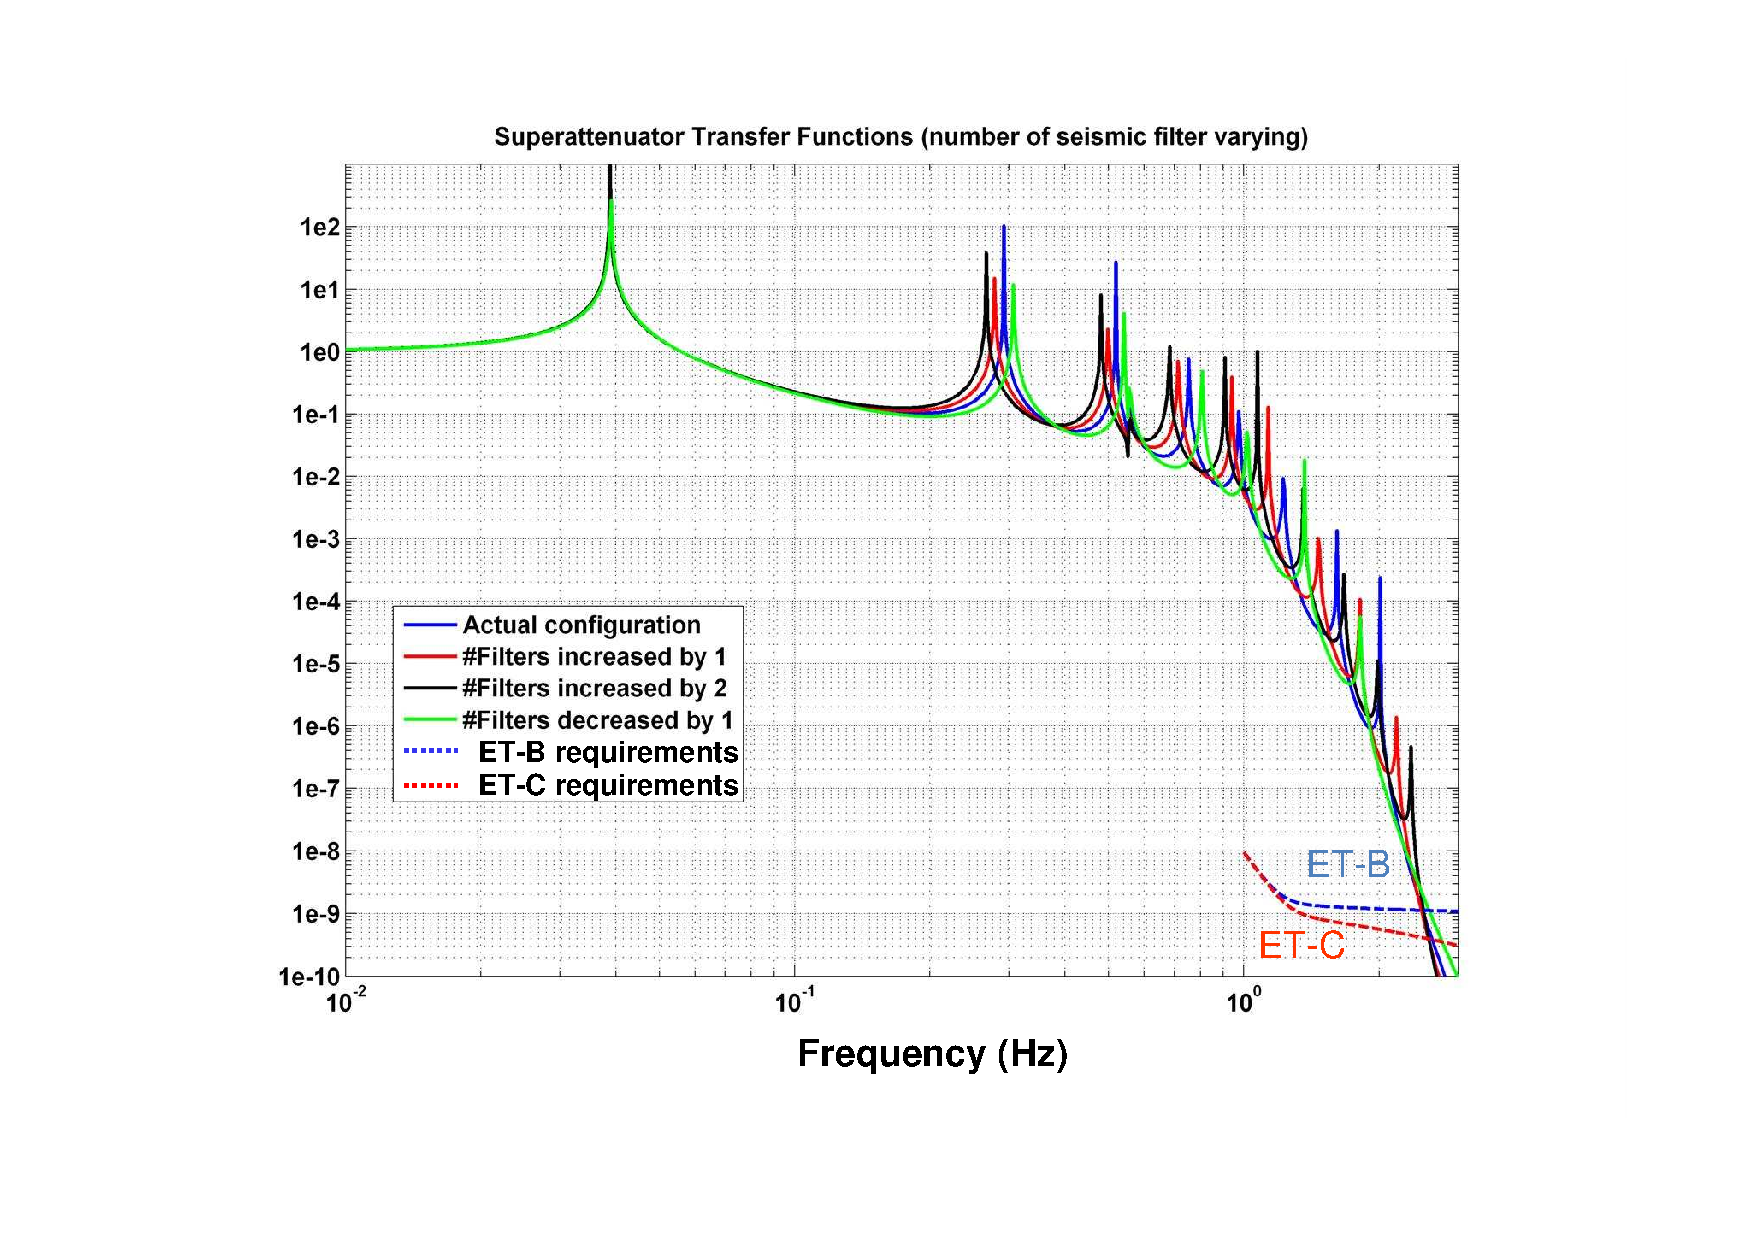
\includegraphics[width=0.9\textwidth]{Detector/SASandSUS/SuspensionSystems/Suspension_Figures/Par4-Fig1.pdf}
			\caption{Simulation results of the SA horizontal transfer function with the present chain length (9 m). Changing the number of (``equal-spaced'') filters the resulting horizontal transfer function is compared with the ET requirements (for High Frequency---\emph{ET-B}---and low frequency or ``xylophone'' configuration---\emph{ET-C}). Adding or removing filters along the chain length do not have remarkable role in the positioning of the cross-over frequency with the requirements.}
\label{Par4Fig1}
	\end{center}
\end{figure}
%
An important preliminary conclusion of the abovementioned design study is that, fixing the length and the number of mechanical filters, the optimal configuration (i.e.\ that one minimizing the cross-over frequency or maximizing the attenuation performance at 2\,Hz) is that one where the filters are separated along the chain by the same distance. This "equal-spaced" configuration represents the optimal one even because the vertical transfer function is not influenced by the filter positioning along the chain. Moreover it has been proved that increasing\,/\,decreasing the number of filters or changing their masses does not play a fundamental role in determining the cross-over frequency between the horizontal transfer function and the requirements. The results obtained are plotted in Fig.~\ref{Par4Fig1} and Fig.~\ref{Par4Fig2} while in the corresponding captions complementary information is available.  
%
\begin{figure}[t]
	\begin{center}
		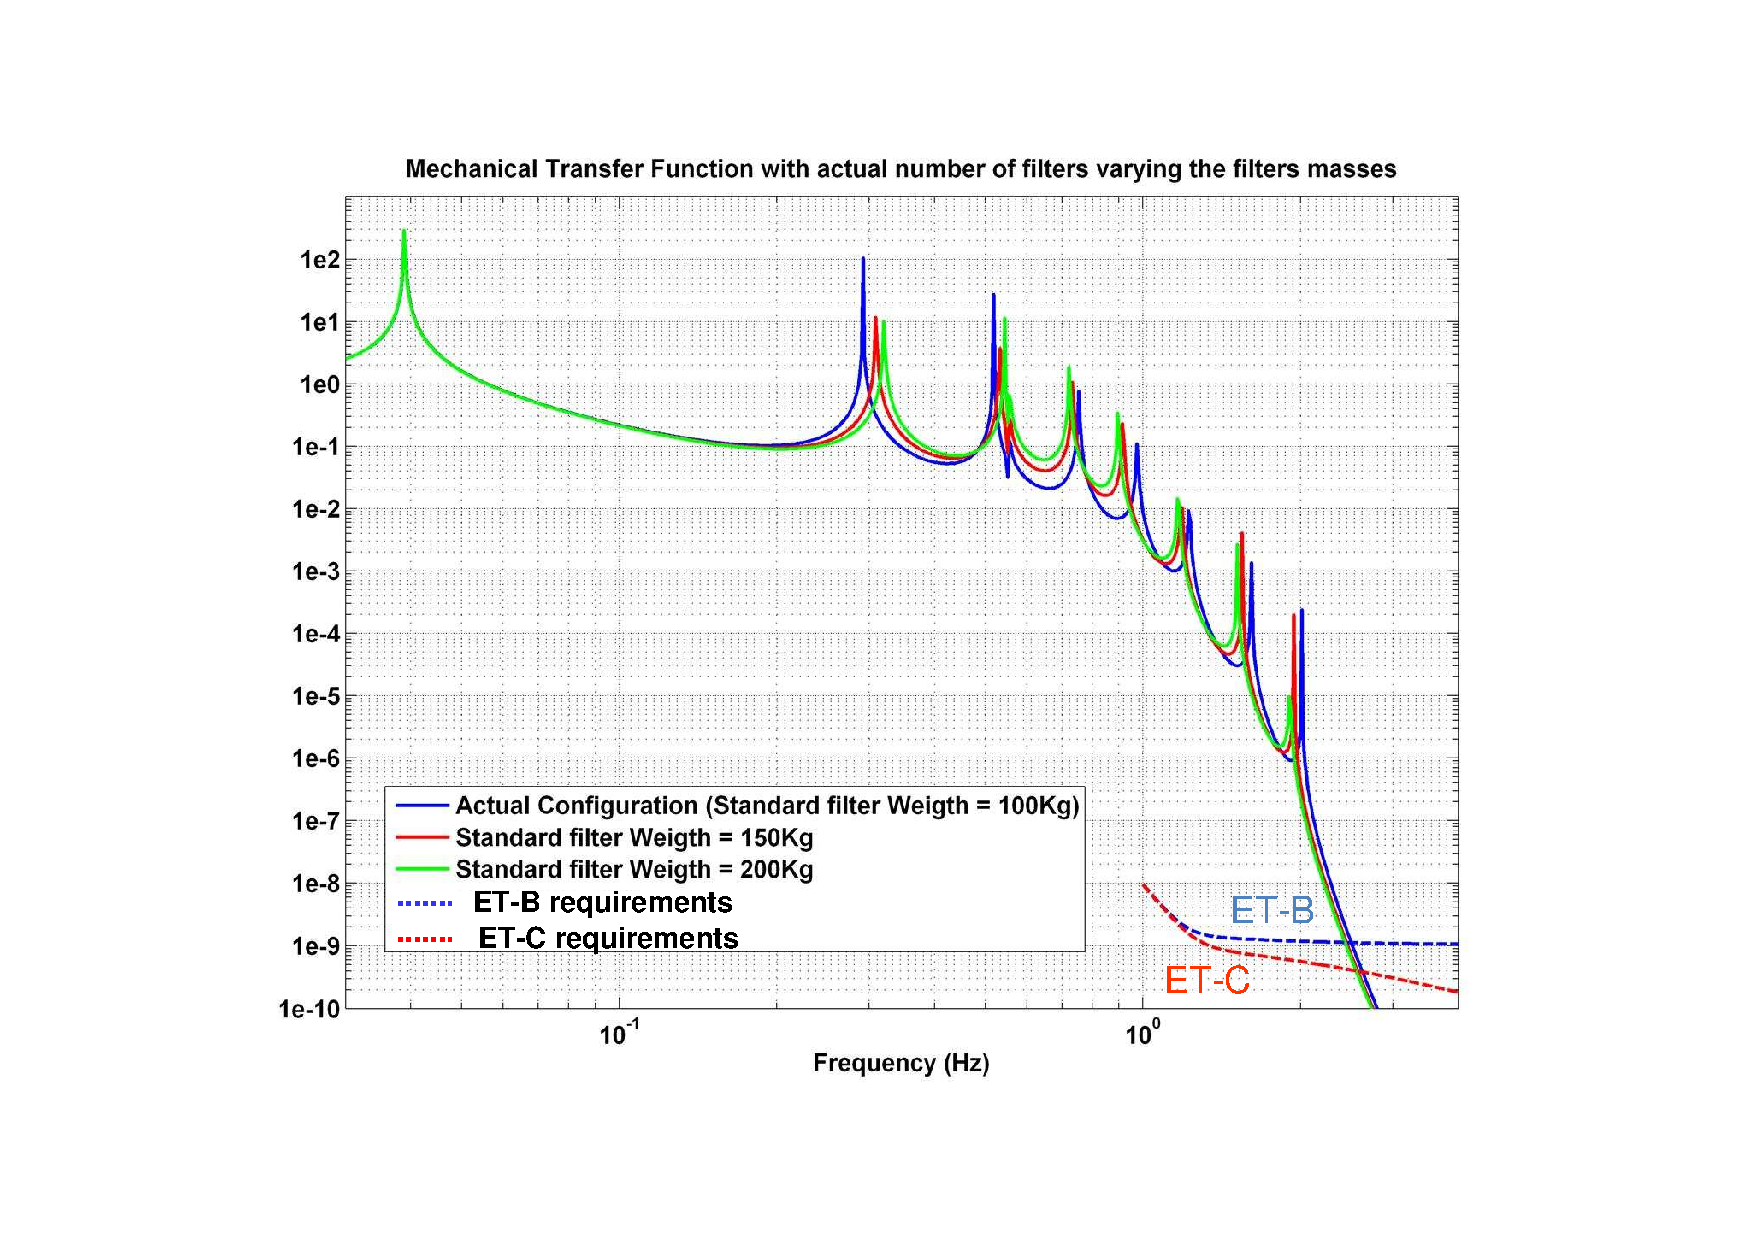
\includegraphics[width=0.9\textwidth]{Detector/SASandSUS/SuspensionSystems/Suspension_Figures/Par4-Fig2.pdf}
			\caption{The horizontal transfer function of the present \emph{SA} (6 filters weighting 100\,kg each one for a total length of about 9\,m) is compared with the same transfer function changing the mass of each filter (150\,kg and 200\,kg). Also in this case the cross-over frequency with the ET requirements is not remarkably affected by the change of the filter mass.}
\label{Par4Fig2}
	\end{center}
\end{figure}
%
\begin{figure}[t]
	\begin{center}
		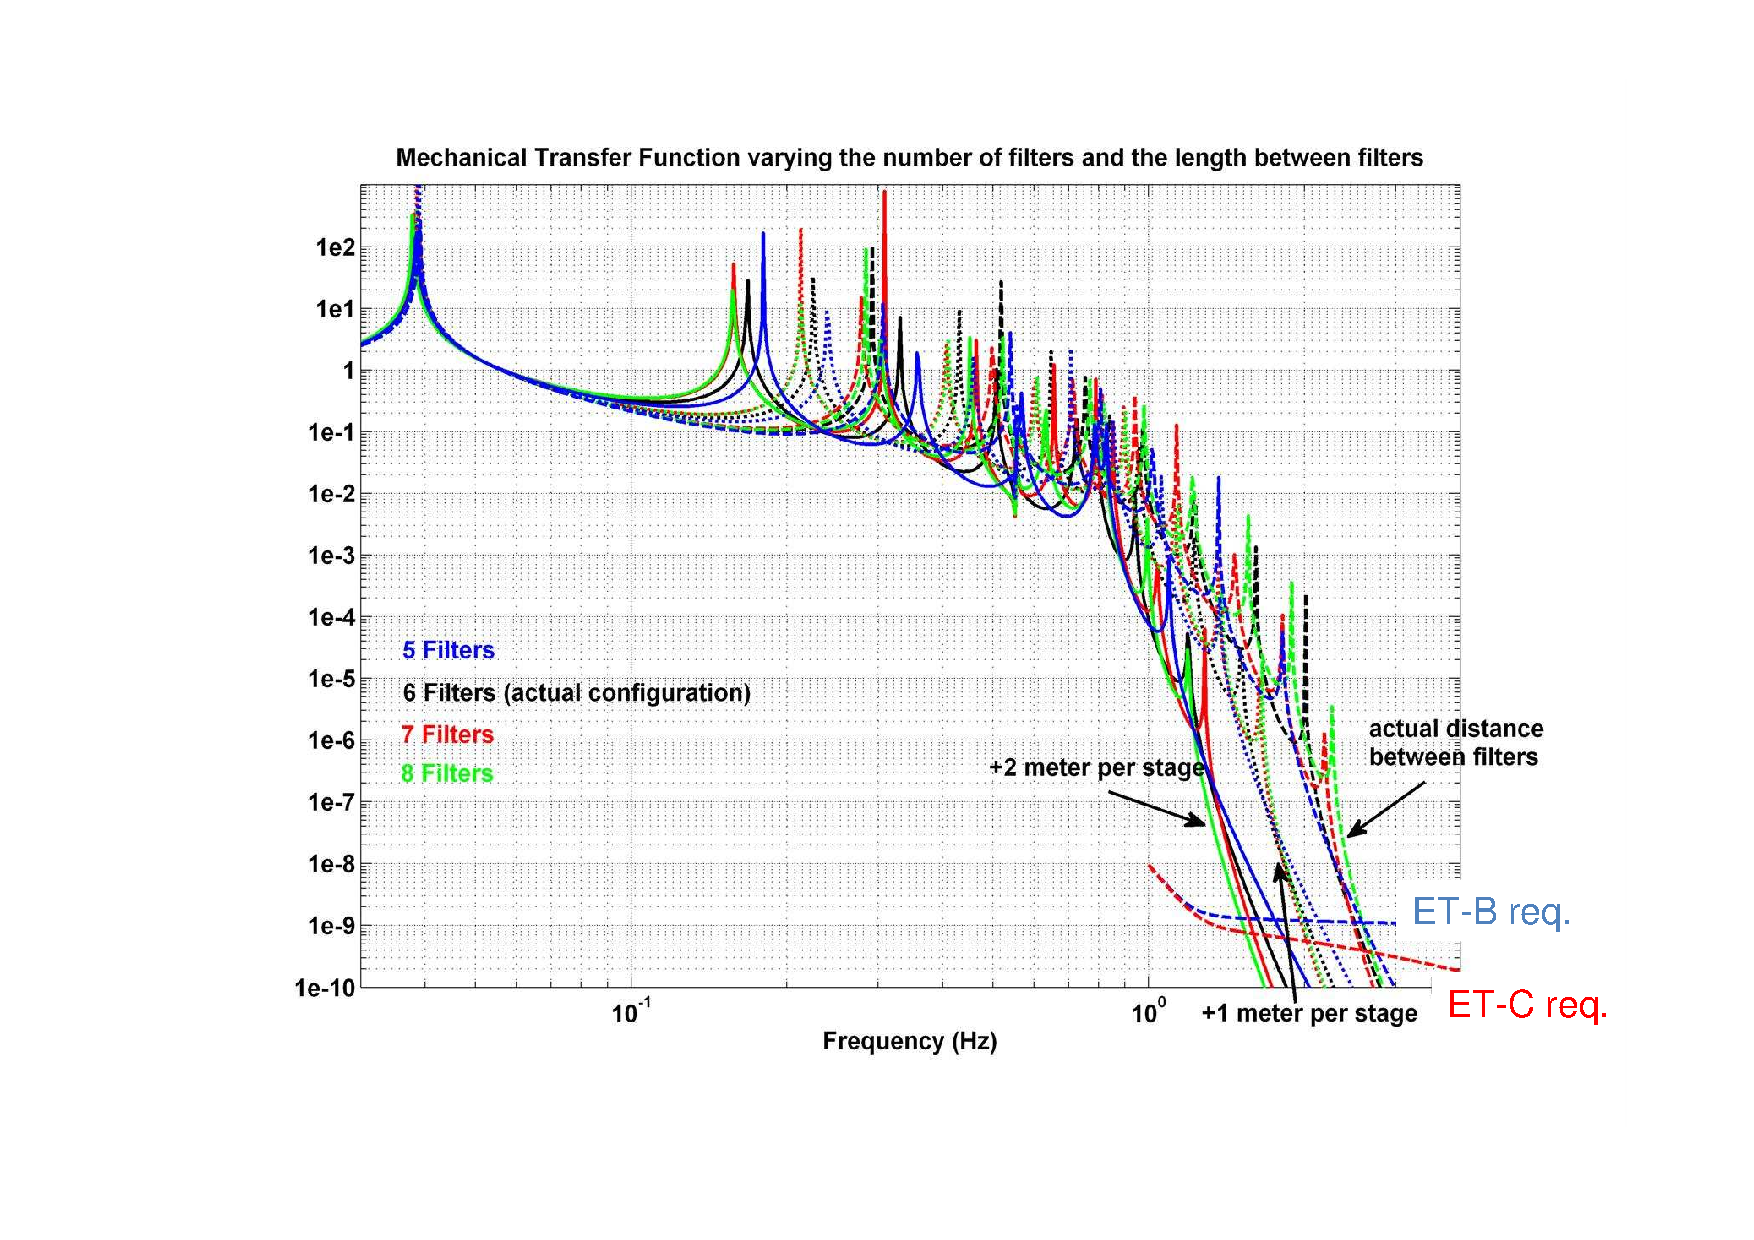
\includegraphics[width=0.9\textwidth]{Detector/SASandSUS/SuspensionSystems/Suspension_Figures/Par4-Fig3.pdf}
			\caption{Simulation results for different configurations. The horizontal transfer function of the \emph{SA} is plotted changing the number of filters and keeping fixed their relative distances ("equal-spaced" geometry) along the chain (changing, as a consequence, the full length of the SA).}
\label{Par4Fig3}
	\end{center}
\end{figure}
%
The only way to move in the low frequency region the cross-over frequency extending the Einstein Telescope bandwidth below 3 Hz, is to increase the SA chain total length. The simulation results for different configurations can be found in figure~\ref{Par4Fig3} and described in~\cite{Braccini2010March1-3}, while the best solution seems to be represented by a SA with 6 filters and a total length of 17\,m (identical the Virgo configuration, where 5 mechanical filters suspended from an horizontal pre-isolator stage plus the marionette are assembled forming a filter chain about 9\,m long). As shown in Fig.~\ref{Par4Fig4}, with this solution the cross-over frequency has been placed around 1.7--1.8\,Hz, that is considered enough for our purpose. Indeed, Newtonian noise and other technical noise are assumed to prevent an effective detection above a couple of Hz.
%
\begin{figure}[t]
	\begin{center}
		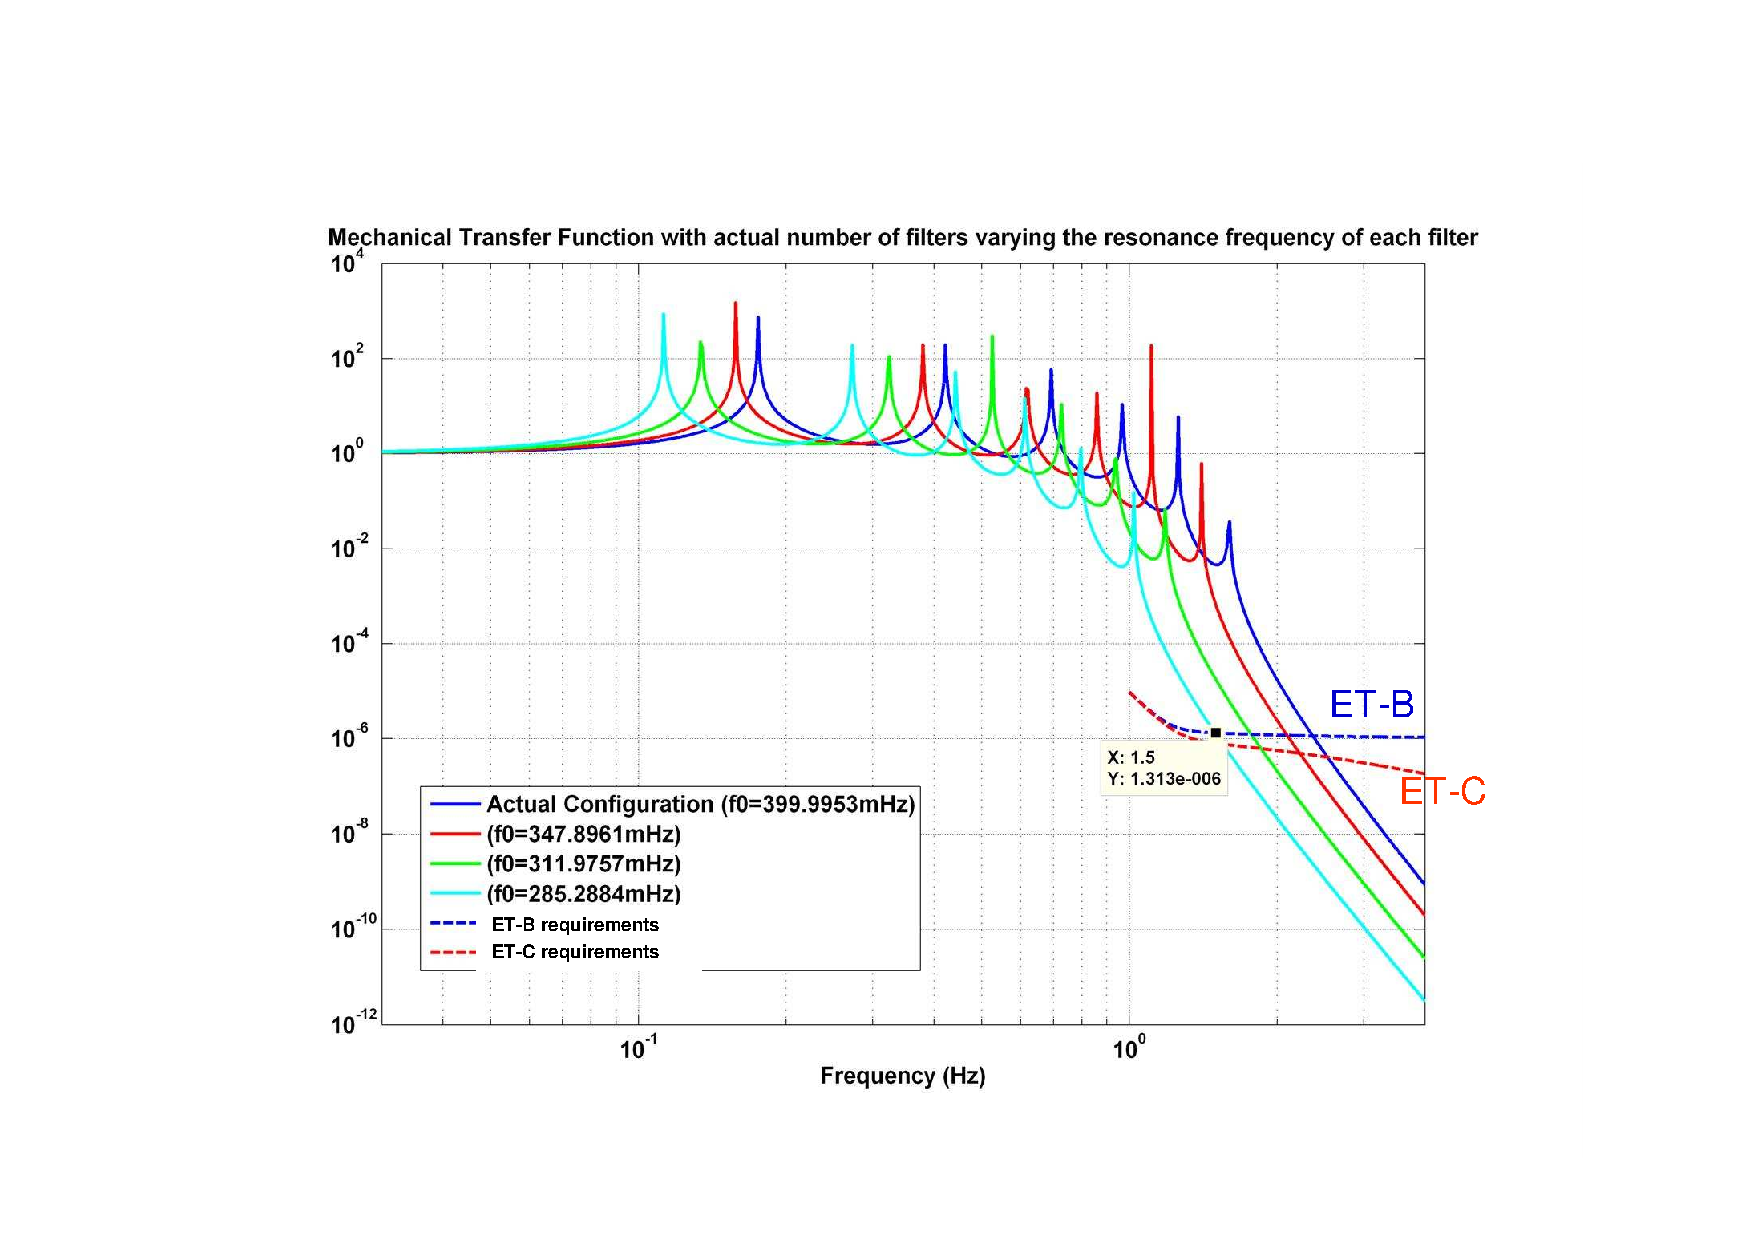
\includegraphics[width=0.9\textwidth]{Detector/SASandSUS/SuspensionSystems/Suspension_Figures/Par4-Fig5.pdf}
			\caption{Vertical Transfer Function of the SA considering the six stages (as it is now, i.e.\ with the pre-isolator or ``Filter Zero'' plus other five mechanical filters). The different curves have been obtained changing the filter vertical resonant frequency. With filters working around 300\,mHz it is possible to move the cross-over below 2\,Hz.}
\label{Par4Fig5}
	\end{center}
\end{figure}
%
With this configuration, the vertical cut-off frequency of the whole system is set below 1.8\,Hz by tuning each mechanical filter having the main vertical frequency around 300\,mHz (see Fig.~\ref{Par4Fig5}). The corresponding vertical transfer function is plotted in Fig.~\ref{Par4Fig4}. Since the residual seismic noise along the vertical direction, at the level of the mirror, is expected to limit the Einstein Telescope sensitivity again around 1.7--1.8\,Hz, a coupling factor of $10^{-3}$ has been considered. This is due to the fact that the Earth curvature makes plumb lines at a 10\,km distance not parallel each other. At least one mirror has to be inclined with respect to the local plumb line performing the alignment of the cavities. This transmits the residual vertical mirror motion along the beam with the mentioned coupling factor ($10^{-3}$).
%
\begin{figure}[t]
	\begin{center}
		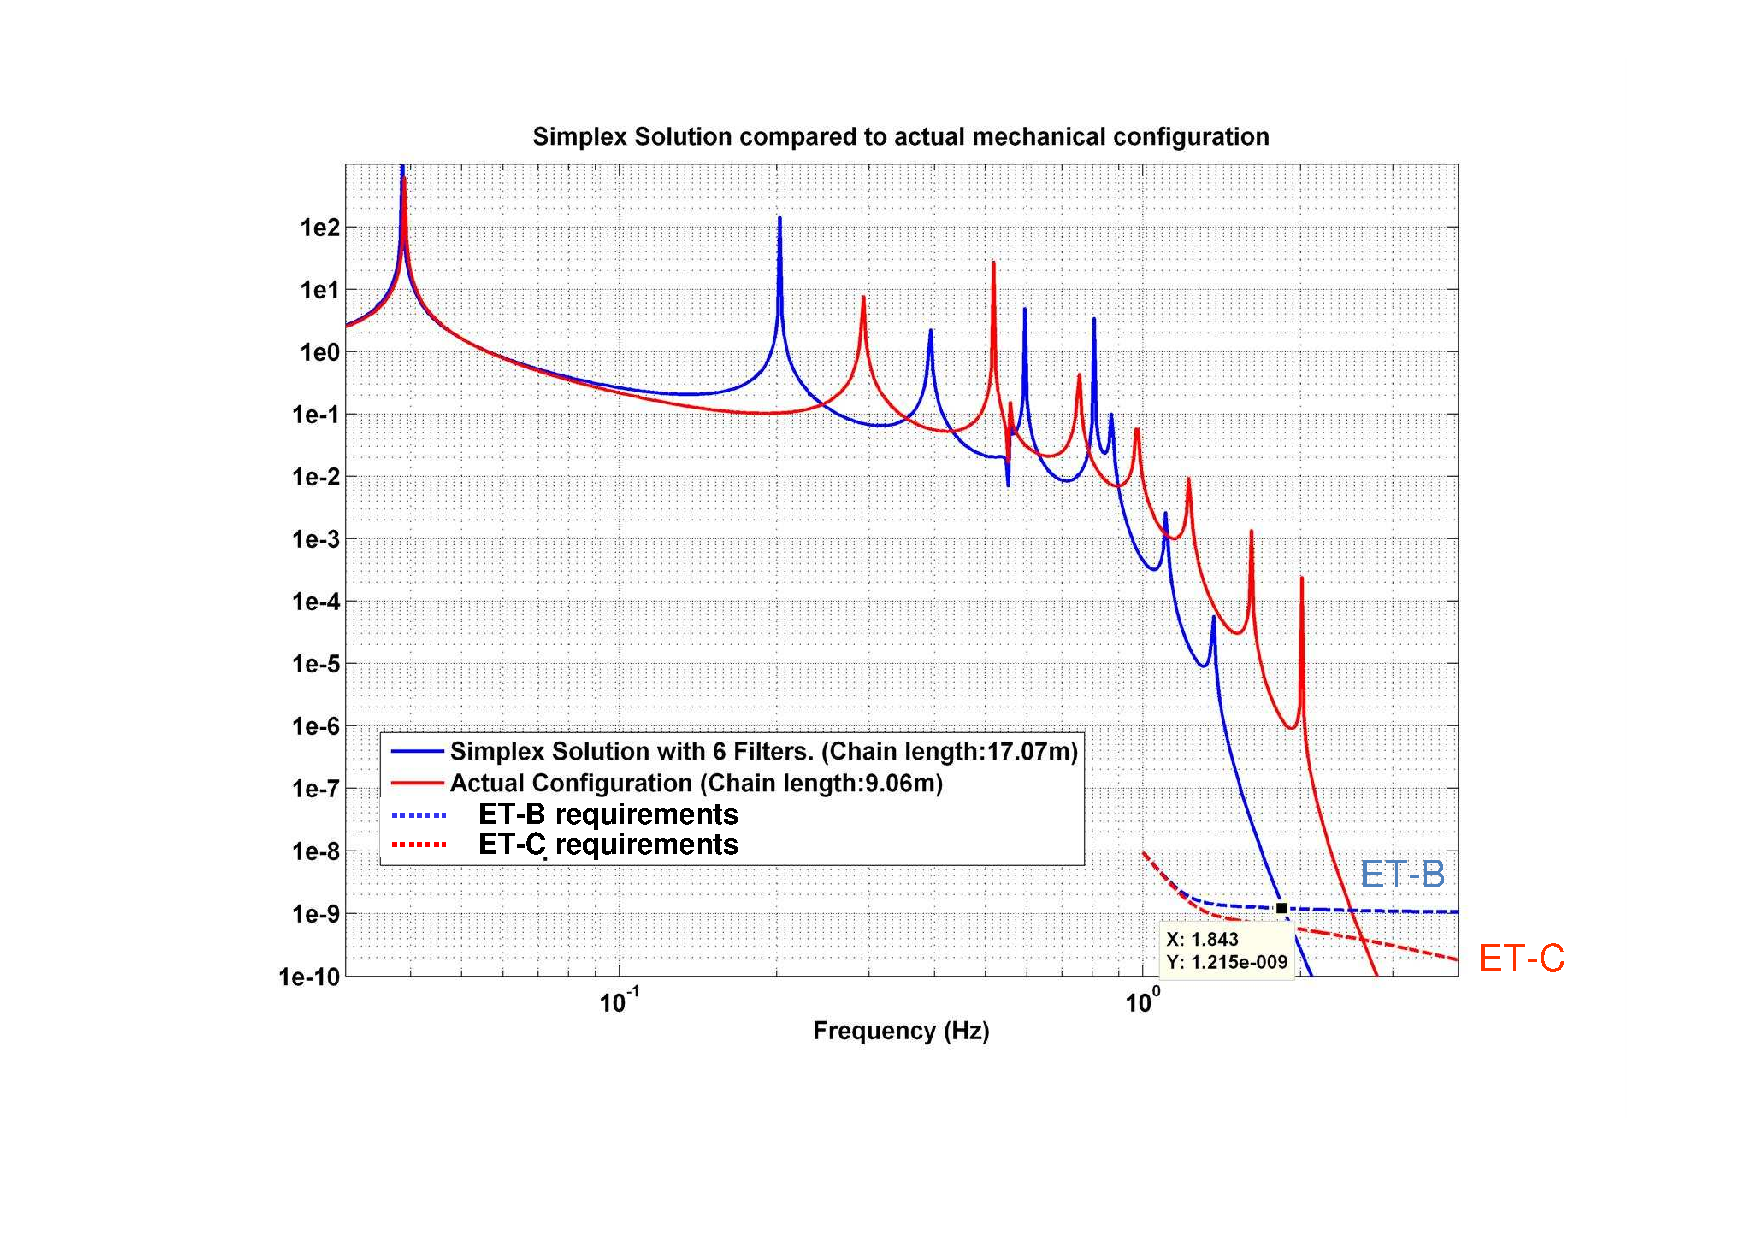
\includegraphics[width=0.9\textwidth]{Detector/SASandSUS/SuspensionSystems/Suspension_Figures/Par4-Fig4.pdf}
			\caption{The proposed reference solution for the $SA$ configuration of the Einstein Telescope. Other slightly different configurations are discussed in \cite{Braccini2010March1-3}.}
\label{Par4Fig4}
	\end{center}
\end{figure}
%
Since years in Virgo many mechanical filters with a cut-off frequency of around $300$ $mHz$ \emph{Superattenuators} are  in operation  with an excellent stability. By using the Virgo interferometer data, it has been observed that the long-term change of the chain main resonant frequencies induced by the temperature variation under vacuum are 
well inside the line-width of the chain vertical resonances. No effect on the interferometer control is due to this potential disturbance. Moreover, even if the temperature variations induce a motion of the suspension chain and then a slow vertical displacement ({\it {breath}}) of the mirror (a few $mm$ per $^{\circ}C$ is the measured 
value for the Virgo \emph{Superattenuator}), this effect is well within the specifications of any interferometer (vacuum tank provides an excellent temperature stability - fraction of $^{\circ}C$ peak to peak).
The standard SA, presently in operation on the Virgo interferometer, is already well inside the third generation specifications from this point of view too.

In addition, it is important to remind that the requirements in the tens of Hz range are less stringent in Einstein Telescope than in Advanced Virgo (see section 4.1.1.a) and thus, fixing to six (a choice lead by the reduction of the cross-over frequency) the number of filters, a better attenuation performance in the high frequency range is not necessary anymore since the safety margin is large enough in Advanced Virgo and even larger in an underground environment. In conclusion, a SA $17$ $m$ high with 6 magnetic anti-spring filters ("equal-spaced" configuration) tuned with a vertical cut-off frequency around 300 $mHz$, represents the reference solution for the Einstein Telescope. 

{\bf Possible alternatives to the baseline}

There are two main reasons which push for seeking a different approach:
\begin{itemize}
    \item the 17m Superattenuator is not sufficient to push the seismic wall down to 1 Hz, which is the ET target;
    \item it could be convenient to reduce the Superattenuator height to ease the constraints on the height of the caverns.
\end{itemize}


A possible alternative to be investigated could be coupling a Superattenuator to an inertial platform controlled in 6 d.o.f.: this configuration would make use of a combination of the technologies and expertise developed in the GW field so far. One could imagine, for instance, the inertial platform being the base of the Superattenuator. This kind of approach was envisaged already in Virgo: the Superattenators are realized on a rigid platform resting on 3 elastic feet which can be actuated by piezos. This had been designed in order to be able to perform an active control of the ground tilt. The ET design should extend this concept in order to allow also for horizontal control.




%{\bf Mechanics of the suspension upper stages}

%The suspension upper-stages are primarily required for the reduction of input vibration within the sensitive band. They are also often used for actuation and damping. 

%\textit{In Virgo, this is all filters between Filter Zero and the Marionette, in LIGO this is the 'top' and 'UIM' masses of the Quads.}



{\bf Sensor development}

The seismic isolation systems will require the development of new sensors not currently deployed in-vacuum. At the minimum, this will include some kind of inertial rotation sensor to enable tilt-control at frequencies at and below the micro-seismic peak, and displacement sensors to allow damping of suspension modes without injecting noise.
In general, the lower seismic noise intensity in the underground site will naturally require accelerometers with a lower proper noise. 



\subsection{Test Mass Suspension Systems}
\label{Sec:SUS}
https://www.overleaf.com/5857319888dfyxsfqvsgpx

hal: this url does not exist. Did you mena:
https://www.overleaf.com/project/5d40a8fe67993a7c805ef910 ?

\section {Newtonian Noise and Environmental noise}
% author Jan Harms?

\subsection {Newtonian Noise Cancellation}
\label{Sec:NewtonianNoise}
\FloatBarrier
\label{sec:mitigateNN}
Local environmental mass-density fluctuations produce so-called Newtonian noise (NN) in a gravitational-wave detector through direct gravitational coupling with its test masses. Density perturbations can be associated with seismic, sound, temperature, and humidity fields, but also be produced by moving and vibrating objects. Newtonian-noise cancellation comprises techniques where auxiliary sensors are deployed to monitor sources of density perturbations, and their data are then used to produce a NN estimate that is being subtracted from the GW detector data.

As described in Section \ref{SiteReq}, the first step of any NN mitigation strategy is to reduce environmental disturbances. For ET, this includes site selection, underground construction, and realizing a low-noise detector infrastructure. However, only if the natural environment is among the quietest in the world, and excess anthropogenic noise can be avoided, then it might be possible to achieve the ET sensitivity target without NN cancellation. Nonetheless, without a detailed understanding of the seismic field, which is hard to obtain even with an extensive site-characterization study, NN modeling uncertainties are significant. It is therefore necessary to include NN cancellation in the R\&D plans.
\begin{figure}[t!]
    \centering
    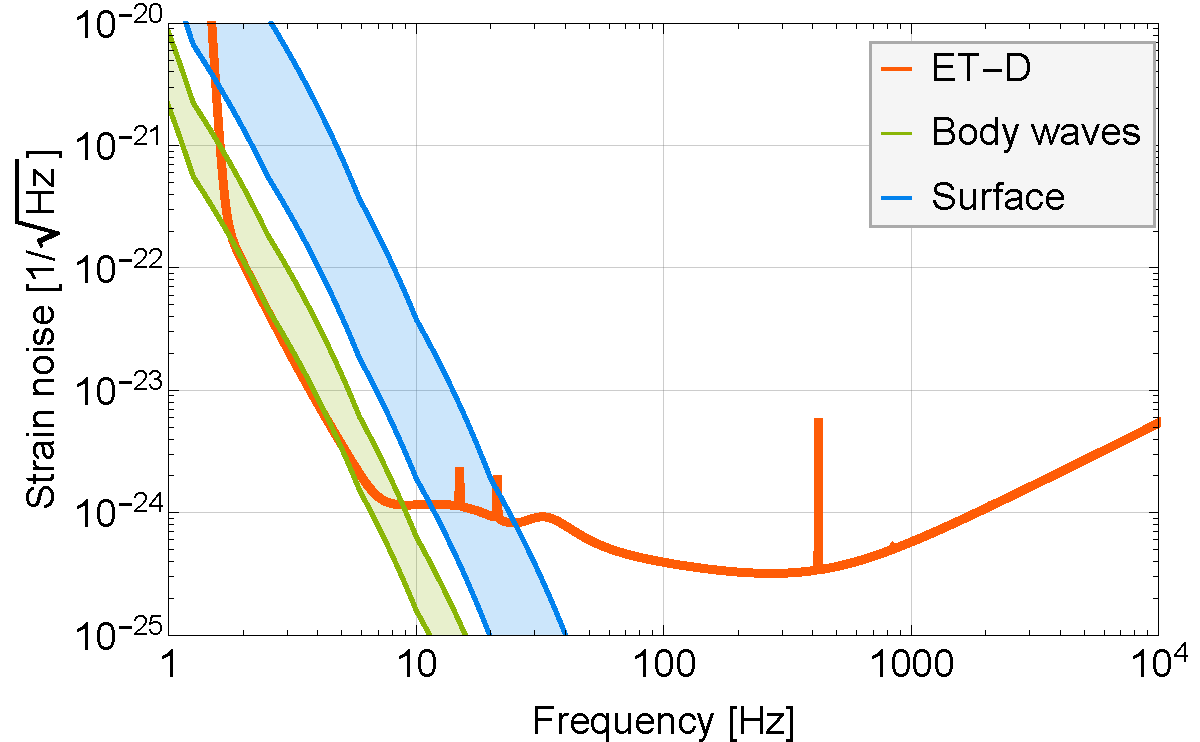
\includegraphics[width=0.49\textwidth]{./Detector/NewtonianNoise/NewtonianNoiseFigures/Seismic_Surf.pdf}
    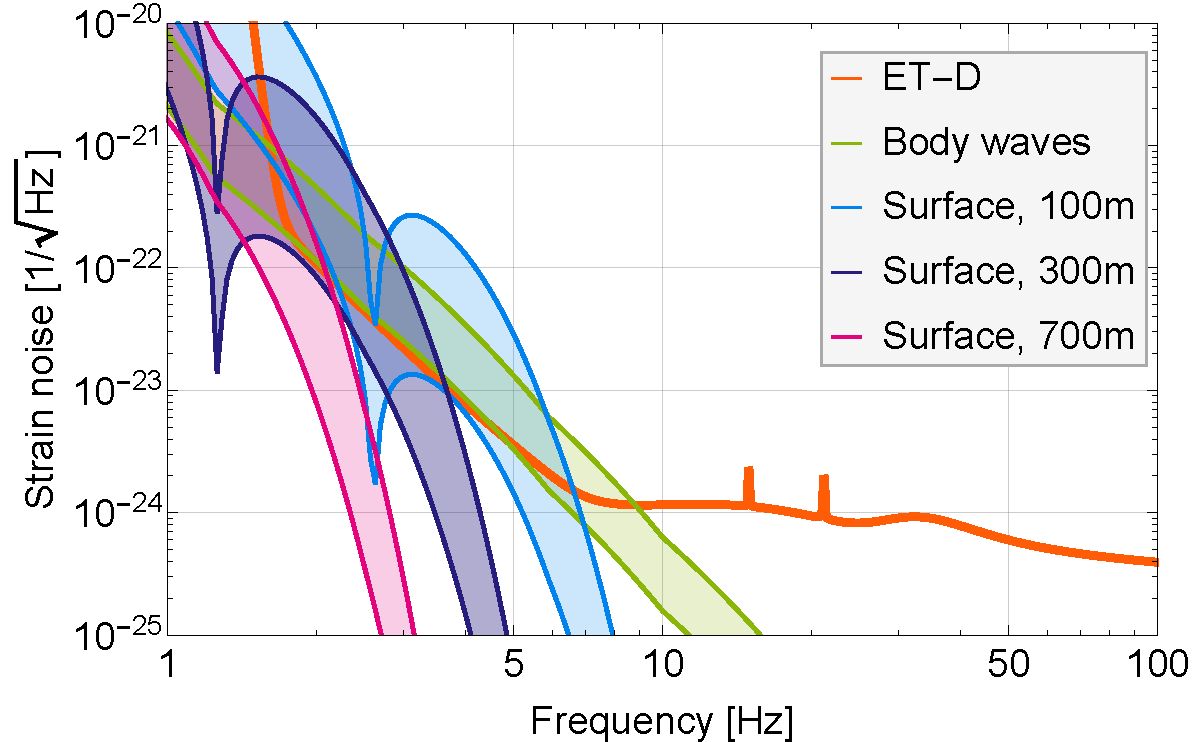
\includegraphics[width=0.49\textwidth]{./Detector/NewtonianNoise/NewtonianNoiseFigures/Seismic_UG.pdf}
    \caption{Estimates of seismic NN for ET. Left: ET constructed at the surface. Right: ET constructed underground. Plot from \cite{BaHa2019}.}
    \label{fig:NNestimates}
\end{figure}

As shown in Figure \ref{fig:NNestimates}, NN from surface waves will be strongly suppressed if the detector is constructed a few 100\,m underground. However, the NN from seismic body waves cannot be avoided at any depth, and it becomes a sensitivity-limiting noise contribution below 10\,Hz. Depending on the quality of the underground site, one still needs to mitigate body-wave NN by up to a factor 10. The range of body-wave NN shown in the two plots assumes that underground seismic spectra are a factor 3 to 12 above the global low-noise model \cite{Pet1993}, and an isotropic field is composed entirely of compressional waves. If it were composed entirely of shear waves, then the NN would be a factor 2 smaller. The prediction of Rayleigh NN (denoted {\it Surface} in the two plots) in underground detectors requires an assumption about the seismic surface spectrum, which is a factor 50 to 1000 above the global low-noise models in the two plots, but also an assumption about the dispersion curve. The slower (and therefore shorter) Rayleigh waves, the stronger is the suppression of associated NN with depth \cite{Har2015}. The dispersion model used for the two plots (Rayleigh wavelength plays a negligible role for NN in surface detectors) yields a Rayleigh-wave speed of 1.5\,km/s at 1\,Hz falling to 300\,m/s at 10\,Hz. There can be significant regional variations, but these values are typical. For the body-wave and Rayleigh-wave field, anisotropy can increase or decrease NN relative to the isotropic level shown in Figure \ref{fig:NNestimates}.

\subsection{Coherent noise cancellation}
\label{sub:Wiener}
The basic idea for noise cancellation is to exploit correlations between NN and data from a set of auxiliary sensors. An effective technique is to use Wiener filters \cite{Orf2007}. They are the optimal linear filters for this purpose provided that all time series are stationary, and they are effective even in the presence of non-stationary features in the data. Wiener filters can be estimates from data. It requires the calculation of correlations between all auxiliary sensors monitoring the environment, which form a correlation matrix $\mathbf C_{\rm SS}$, and between auxiliary sensors and GW detector, which form a vector $\vec C_{\rm SN}$. Since one is mostly interested in the frequency-domain representation of detector noise, correlations are expressed as cross-spectral densities depending on frequency $\omega$. The Wiener filter can then be written
\begin{eqnarray}
		\vec w(\omega)=\mathbf C_{SS}(\omega)^{-1}\cdot\vec C_{\rm SN}(\omega)
		\label{eq:Wiener}
\end{eqnarray}
This filter is applied to discrete Fourier transforms of data from auxiliary sensors, $\vec d(\omega_i)$, to produce an estimate $\hat n(\omega_i)=\vec w(\omega_i)^\dagger\cdot \vec d(\omega_i)$ of NN, which is then subtracted from the GW detector data. In average, the relative suppression of NN by a Wiener filter is given by
\begin{eqnarray}
		\epsilon(\omega)=\sqrt{1-\frac{\vec C^\dagger_{\rm SN}(\omega)\cdot \mathbf C_{\rm SS}(\omega)^{-1}\cdot\vec C_{\rm SN}(\omega)}{C_{\rm NN}(\omega)}},
		\label{eq:residual}
\end{eqnarray}
where $C_{\rm NN}(\omega)$ is the spectral density of NN in the GW detector. This expression tells us that to achieve a good subtraction efficiency, three conditions are to be met:
\begin{itemize}
\item All the sensors should be coupled as much as possible to NN. In other words, the correlation $\vec C_{\rm SN}$ between sensor outputs and GW detector must be large.
\item The correlations between sensors, described by the matrix $\mathbf C_{\rm SS}$, which also include sensor noise on its diagonal, must be small.
\end{itemize}
Designing a NN cancellation system for a GW detector that is yet to be built, only the correlations among auxiliary sensors $\mathbf C_{\rm SS}$ can be measured during a site-characterization campaign. A model is required using the correlations $\mathbf C_{\rm SS}$ to obtain $\vec C_{\rm SN}$ and $C_{\rm NN}$ \cite{CoEA2016a}.

The theory of Wiener filtering does not directly address a major challenge of NN cancellation, which is the optimal placement of auxiliary sensors. This aspect is very important for the cancellation of NN from seismic and atmospheric fields. Analyses of optimal array configurations are important since, even when lacking an accurate understanding of environmental fields, optimization results provide useful estimates of the required number of auxiliary sensors, the required sensitivity of sensors, and an approximate idea of how far from the test masses sensors need to be placed. This aspect is discussed in Section \ref{sub:optimization}.

\subsection{Site properties relevant to Newtonian-noise cancellation}
\label{sub:properties}
Since the Wiener filter is based on correlations in environmental fields, anything that influences these correlations affects NN cancellation. In the following, site properties relevant to seismic and atmospheric NN are briefly described.

\subsubsection*{Seismic fields}
\begin{itemize}
\item {\bf Seismic speed}\; Seismic correlations and correlations of seismic NN between test masses decrease with increasing distance. In frequency domain, this can be quantified in terms of a spatial correlation function $\mathcal F$ that assumes its maximal value 1 when the two seismometers or test masses are sharing the same location. As a function of the separation $L$, one finds for isotropic Rayleigh-wave fields
\begin{eqnarray}
	\mathcal{F}_{\rm NN}=J_{0}(2\pi L/\lambda)-J_{2}(2\pi L/\lambda),\quad \mathcal{F}_{\rm seis}=J_{0}(2\pi L/\lambda).
	\label{eq:geometrical}
\end{eqnarray}
As is intuitively clear, how quickly correlation decreases with increasing distance $L$ depends on the length $\lambda$ of a Rayleigh wave. The first zero of the seismic correlation is at a distance of about $0.4\lambda$. Correlations of NN between two test masses of one arm separated by several kilometers can be neglected. Due to equation (\ref{eq:residual}), seismometer arrays used for NN cancellation ideally have diameters similar to the length a Rayleigh wave. 

\item {\bf Wave polarizations}\; Seismic-wave polarizations play a major role in NN cancellation. The two main polarizations are shear and compressional waves, and Rayleigh surface waves are a so-called inhomogeneous (amplitude decreasing exponentially with depth) extension of a superposition between these two polarizations. The composition of the seismic field in terms of wave polarizations varies between sites, and depends on local geology as well as on the type and location of seismic sources. All polarizations produce NN either through compression of the medium or by displacement of surfaces and interfaces.

If only one wave polarization is present at a time, then it is almost trivial to cancel associated NN \cite{Har2015,HaVe2016}. A mix of wave polarizations can however make it very difficult to cancel a significant amount of NN \cite{HaVe2016,BaHa2019}. The issue is that correlations between seismometers and test mass decrease more quickly with distance when multiple polarizations are present, which hampers efficient noise cancellation as pointed out in Section \ref{sub:Wiener}. As a consequence, a larger number of seismometers is required to be able to be distinguish between polarizations and be susceptible to the correlations of each wave type. 

\item {\bf Seismic sources}\; The distribution and type of seismic sources both influence the composition of a seismic field. Most important to know is whether seismic sources are local or distant, and whether they are underground or at the surface. Some sources might not even fall into a clear category if it is for example a surface structure anchored to a deeper part of the ground. With respect to environmental noise, it is one of the most important tasks of a site-characterization campaign to identify as many seismic sources as possible. A NN cancellation scheme can be greatly simplified or be made significantly more effective if understanding about the seismic sources is used. Furthermore, excess noise produced by the infrastructure of the Einstein Telescope will also pose additional challenges for the design of a NN cancellation system. 

\item {\bf Local topography and geology}\; Two-point correlations of the seismic field can be affected by topography and geology. Generally, seismic-wave reflections from surfaces and interfaces cause conversions between wave polarizations. Scattering from non-planar structures can also give rise to local field components that strongly decay with distance. These local components are very similar in nature to the near-field of seismic sources. In the presence of significant geological heterogeneities or rough surface topography, it is therefore more challenging to collect all information required to design seismometer arrays for efficient NN cancellation \cite{CoHa2012}. Especially in relatively noisy environments with elevated NN where more efficient cancellation of NN might be required, site characterization should therefore assess geological properties and topography also in the context of NN cancellation.

\end{itemize}

\subsubsection*{Atmospheric fields}
Avoiding NN from the atmosphere is an important reason to construct the Einstein Telescope underground. In Section \ref{sec:envnoise}, some of the complexity of atmospheric fields and how they produce NN are described. There are serious practical challenges to design a cancellation system for atmospheric NN. 

\begin{itemize}
\item {\bf Wind noise}\; The variety of phenomena makes the monitoring of the atmosphere a challenging task. One strategy for NN cancellation would be to monitor sound, wind speed, temperature and humidity fields. Sound is typically measured with microphones. However, pressure fluctuations produced by turbulent flow in the vicinity of a microphone can mask an underlying sound signal \cite{Gre2015}. This contribution is often called wind noise. Clever sensor design, averaging pressure signals over some baseline, or constructing wind shields can prove effective \cite{Ell1972,WaHe2009,NoEA2014}. However, when it comes to an order of magnitude suppression of NN from sound, then even a small incoherent contribution to signals from wind noise can be detrimental. For this reason, entirely new approaches need to be considered. 

\item {\bf LIDAR}\; LIDAR (derived from \emph{light} and \emph{radar}) technology has been applied to investigate microscale physics in the atmospheric boundary layer. It consists of a laser beam that scatters back from the atmosphere carrying information about the presence of certain molecules, or wind speed \cite{CLN2004}, temperature \cite{Beh2005}, etc. Volumetric observations can be performed to characterize the evolution of entire fields. It is conceivable that a LIDAR system can be developed in the foreseeable future to cancel at least modest amounts of wind-driven NN associated with temperature and humidity fields. However, atmospheric density perturbations due to sound are orders of magnitude weaker in the ET observation band, which makes it extremely challenging to develop a LIDAR to monitor sound fields.

\item {\bf Cavity atmosphere}\; Potentially significant NN contributions can come from the sound field inside the cavities hosting the test masses of the Einstein Telescope \cite{FiEA2018}. Due to the absence of fast air currents, wind noise in microphones located inside the cavity will be strongly reduced, and high-precision sound monitoring would be possible. At the same time, absence of fast air currents also means that all forms of cavity atmospheric NN driven by wind, i.e., associated with temperature and humidity fields, will be negligible. This means that cancellation from cavity atmospheric NN should be possible using an array of microphones.
\end{itemize}

\subsection{Optimized sensor arrays for seismic NN cancellation}
\label{sub:optimization}

Another important point to understand is how the subtraction procedure improves with the number of sensors, and how much it is sensitive to a non optimal placement of the sensors. This is important because in a practical implementation, the possibility of optimizing the placement of underground sensors will be limited. 

Optimized seismometer arrays were initially studied for the cancellation of NN from Rayleigh waves \cite{DHA2012,Har2015,CoEA2016a}, and more recently from body waves \cite{BaHa2019}. Array optimization was based on simplified models of the seismic field in all these publications, which means that the calculated array configurations are not of direct use for NN cancellation in real environments. However, the total number of seismometers and the seismometer sensitivity required to achieve a certain cancellation performance are less dependent on the model of the seismic field \cite{CoEA2016a}. 

Accordingly, Fig.~\ref{fig:residualN} gives an estimate of the required number of seismometers to cancel a certain amount of body-wave NN provided that they assume their optimal positions. 
\begin{figure}[t!]
	\begin{center} 
		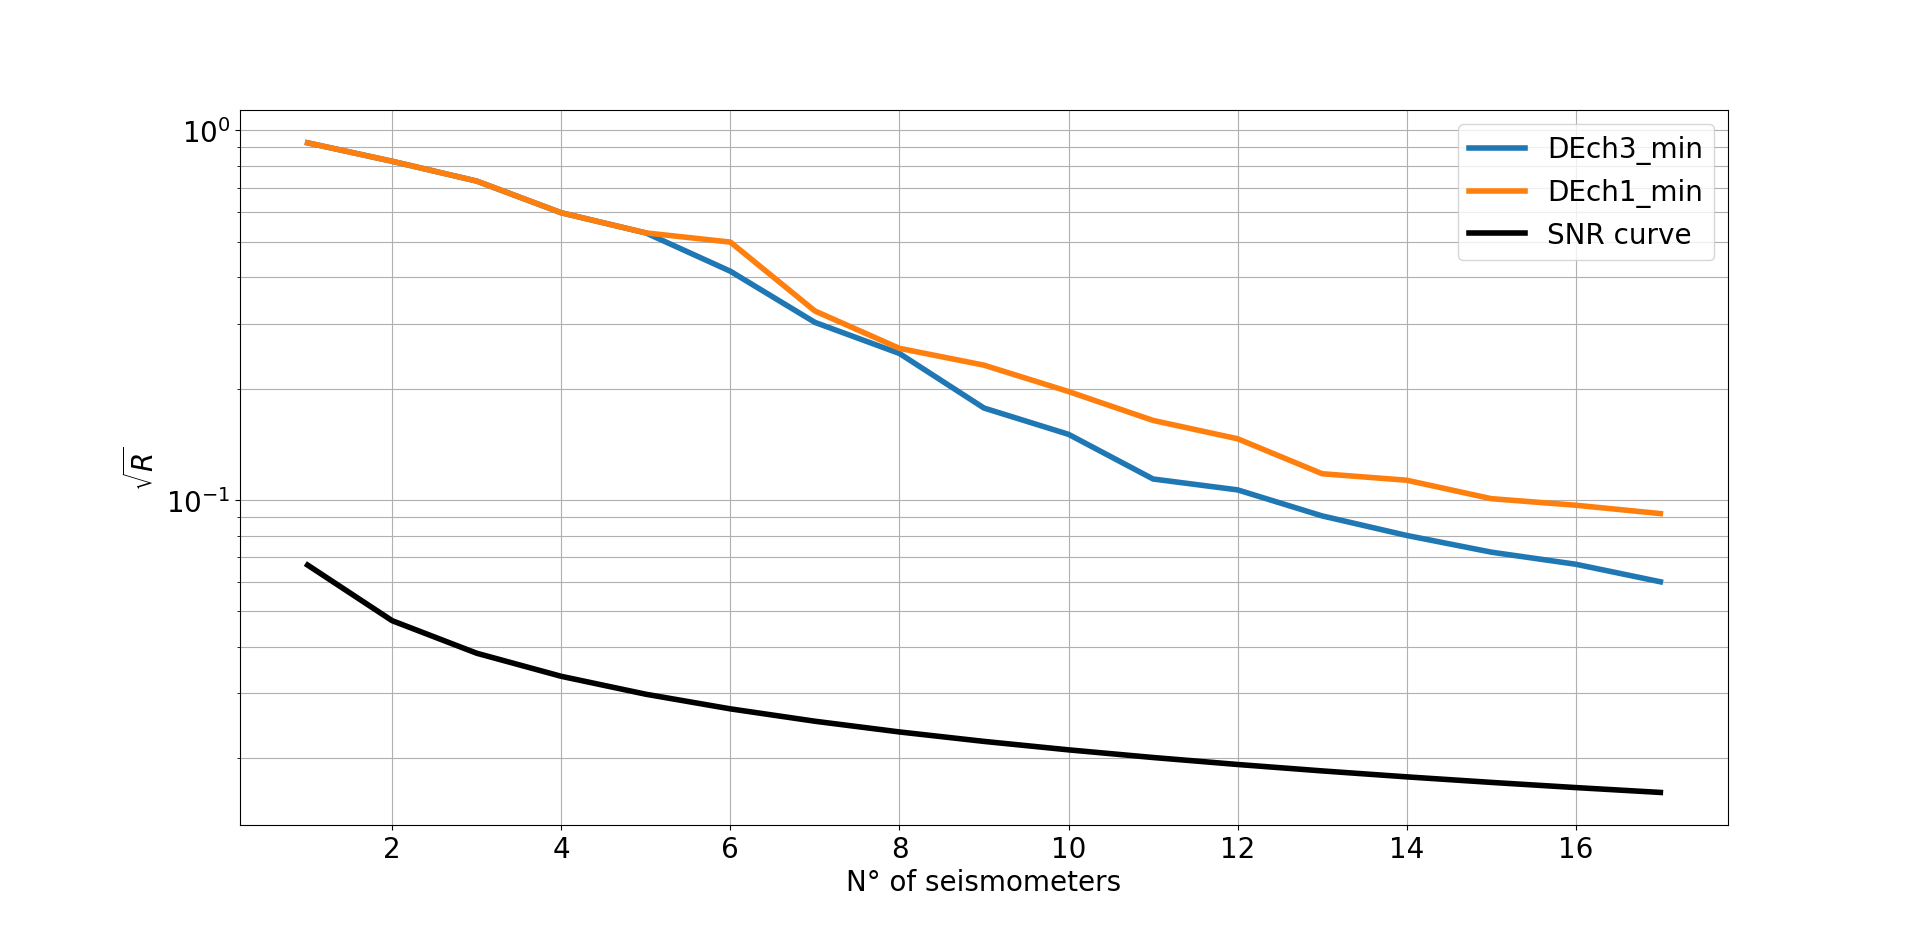
\includegraphics[width=0.7\textwidth]{./Detector/NewtonianNoise/NewtonianNoiseFigures/SNR_ch3.png} 
		\caption{Suppression of body-wave NN as a function of number of seismometers with optimal placement. The seismometers measure seismic signals with an SNR of 15. The black curve shows the lowest possible residual determined by the seismometer SNR without considering properties of the seismic field. Plot from \cite{BaHa2019}.} 
		 \label{fig:residualN} 
	\end{center}
\end{figure}
About 15 seismometers are required to achieve a factor 10 suppression. It should be emphasized that this result depends to some extent on the relative contributions of compressional waves and shear waves to the seismic field. For these results, it is assumed that compressional waves constitute 30\% of the seismic power-spectral density. Less seismometers are required if one polarization greatly dominates over the other. These instruments need to be deployed in boreholes, and the number 15 is per test mass. 

In this context, one can now address the question how accurately the seismometers need to be placed with respect to their optimal locations. While direction and vertical drilling technology has become increasingly accurate \cite{MCZ2016}, significant deviations from optimal drilling are to be expected, which results in sub-optimal seismometer placements. Figure \ref{fig:errorNN} shows the residuals that can be achieved with sub-optimal seismometer placement. 
\begin{figure}[t!]
	\begin{center} 
		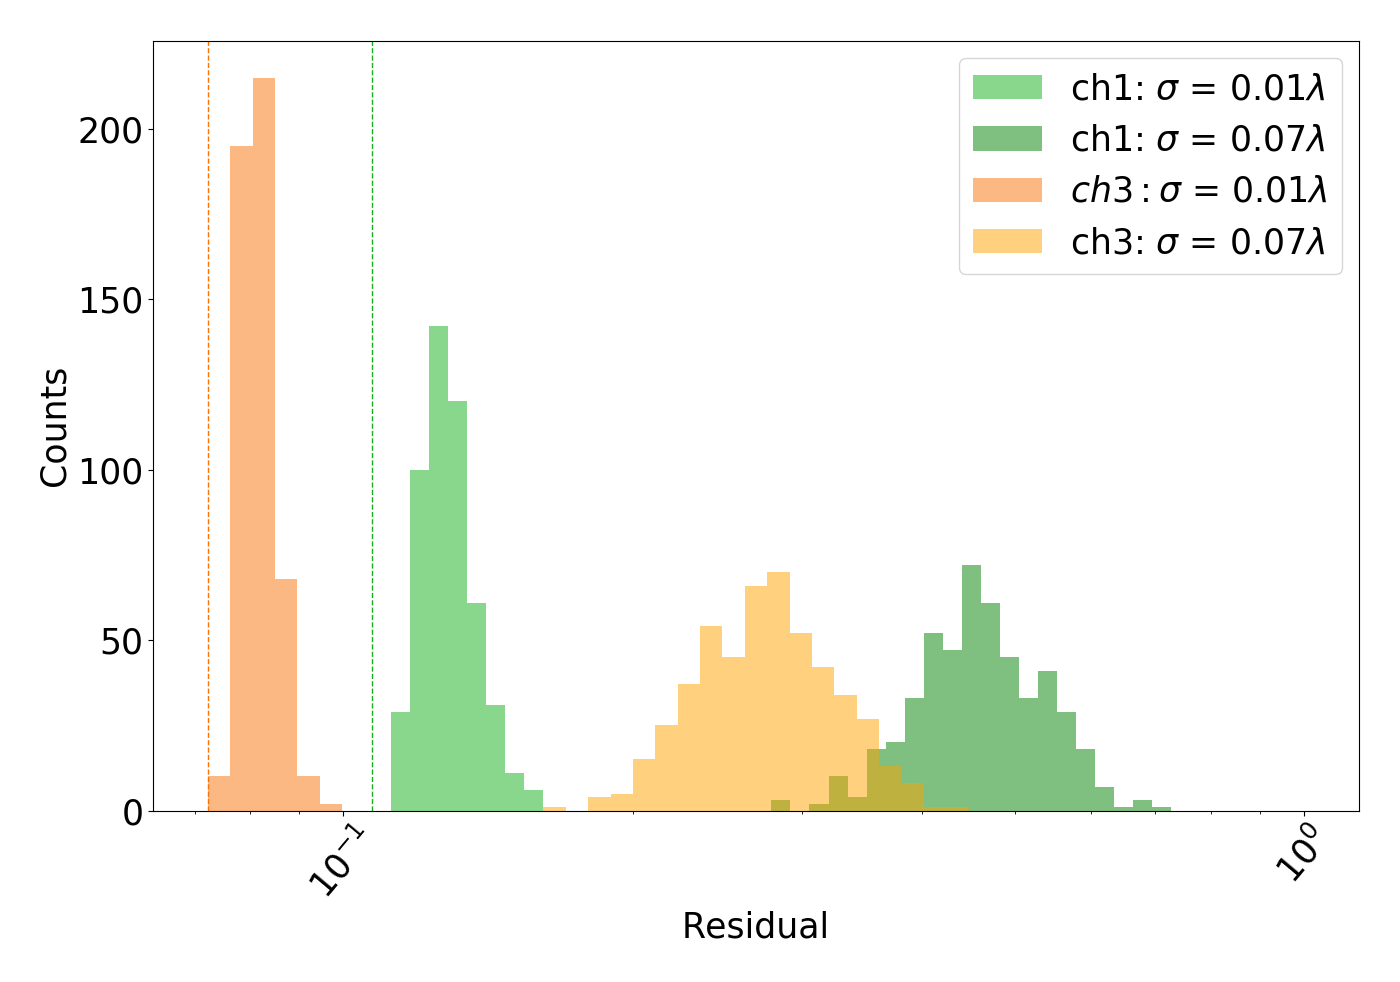
\includegraphics[width=0.7\textwidth]{./Detector/NewtonianNoise/NewtonianNoiseFigures/errorbody.png} 
		\caption{Suppression of NN from body waves with 15 single-axis (ch1) and three-axis (ch3) seismometers. Sensor locations of 500 arrays for each histogram are derived from the optimal array by adding random numbers to all optimal coordinates drawn from Gaussian distributions of width $\sigma$. Vertical lines mark the residual of the optimal arrays. Plot from \cite{BaHa2019}.} 
		 \label{fig:errorNN} 
	\end{center}
\end{figure}
To produce this plot, seismometer coordinates were shifted by a random number drawn from a Gaussian distribution of width $\sigma$ specified in the legend relative to the length $\lambda$ of compression waves. Assuming a compressional-wave speed of 4\,km/s, $\sigma=0.07\lambda=28\,$m at 10\,Hz. The corresponding arrays with three-axis sensors (ch3) still achieve a body-wave NN suppression by a factor 3 and better. For boreholes of a few 100\,m, and drill deviation of less than 1 degree, such sensor-placement accuracy is achievable. 

The remaining challenge is to have sufficient observations of the seismic field to be able to accurately calculate the optimal array configurations. In fact, incomplete knowledge of seismic correlations will likely lead to the dominant error in the seismometer placements. This error needs to be minimized by studying in detail the seismic field at the site of the Einstein Telescope also using borehole seismometer installations.


\subsection {Environmental Noise}
